% Source of the journal-format manuscript (Izvestiya RAN, Ser. Geogr., rules of 17.11.2025).
% Citation placeholders and the two bibliography markers are expanded by
% tools/build_article1_journal.py into article1_v8.tex (plain-text author-year citations).
\documentclass[12pt,a4paper]{article}
\usepackage[a4paper,top=2cm,bottom=2cm,left=3cm,right=1.5cm]{geometry}
\usepackage{iftex}
\ifPDFTeX
  \usepackage[T2A]{fontenc}
  \usepackage[utf8]{inputenc}
  \usepackage[russian]{babel}
\else
  \usepackage{fontspec}
  \usepackage{polyglossia}
  \setdefaultlanguage{russian}
  \setotherlanguage{english}
  \defaultfontfeatures{Ligatures=TeX}
  \IfFontExistsTF{Times New Roman}{%
    \setmainfont{Times New Roman}\newfontfamily\cyrillicfont{Times New Roman}%
  }{%
    \IfFontExistsTF{Liberation Serif}{%
      \setmainfont{Liberation Serif}\newfontfamily\cyrillicfont{Liberation Serif}%
    }{\setmainfont{CMU Serif}\newfontfamily\cyrillicfont{CMU Serif}}%
  }
\fi
\usepackage{setspace}
\usepackage{mathtools,amssymb}
\usepackage{graphicx}
\usepackage{booktabs}
\usepackage{array}
\usepackage{caption}
\captionsetup{labelsep=period,font=normalsize,justification=raggedright,singlelinecheck=false}
\usepackage{titlesec}
\titleformat{\section}{\normalfont\bfseries\centering}{}{0pt}{}
\titleformat{\subsection}{\normalfont\itshape}{}{0pt}{}
\titlespacing*{\section}{0pt}{18pt}{6pt}
\titlespacing*{\subsection}{0pt}{12pt}{3pt}
\usepackage[unicode,hidelinks]{hyperref}
\setlength{\parindent}{1.25cm}
\setlength{\emergencystretch}{3em}
\hyphenpenalty=10000 \exhyphenpenalty=10000
\onehalfspacing
\pagestyle{plain}

\newcommand{\Psurr}{P_{\mathrm{surr}}}

\begin{document}

\noindent УДК 551.513

\begin{center}
{\large\bfseries Сопряженность иерархических уровней атмосферной циркуляции как региональный инвариант}

\medskip
{\bfseries Н. С. Сотириади\textsuperscript{*}}

Независимый исследователь, Москва, Россия

\textsuperscript{*}E-mail: n.sotiriadi@gmail.com
\end{center}

\begin{singlespace}
\noindent\textbf{Аннотация.} Спектральный и фрактальный анализ географических полей отвечает на вопрос, на каких масштабах располагаются уровни организации геосистемы. Следующий вопрос касается отношения между уровнями: размещается ли мезомасштабная изменчивость там же, где активен соседний крупный уровень, или независимо от него. По полю относительного вихря на поверхности 850 гПа (реанализ ERA5, 2017--2024 гг.; 12 основных и 27 контрольных областей) построена мера такого отношения -- профиль сопряженности соседних октавных полос масштаба: пространственная ранговая корреляция карт активности двух соседних полос, дополненная превышением над фазовыми суррогатами поля. Проверена гипотеза о том, что профиль является региональным инвариантом в операциональном смысле: различает циркуляционные режимы и воспроизводится между сезонными окнами разных лет и фаз Эль-Ниньо -- Южного колебания. Региональная группировка профилей подтверждена на отложенных окнах и при перестановках внутри страт сезона, года и периода; на долю региона приходится 0.6--0.7 дисперсии профиля. Группировка сохраняется на ступенях, разрешенных реанализом, при равновеликой нарезке территории, во втором реанализе и в свободном модельном расчете без усвоения атмосферных наблюдений. Более высокие значения свойственны тропическому теплому бассейну Тихого океана, бассейну Конго и внетропическим штормовым путям, более низкие -- континентальным областям и Амазонии; бассейны Конго и Амазонии при сходных стандартных характеристиках режима различаются сопряженностью крупных полос. Величина дополняет аппарат районирования характеристикой устройства межуровневых связей; границы ее применимости указаны явно.

\smallskip
\noindent\textbf{Ключевые слова:} иерархическая организация геосистем, инварианты динамической геосистемы, масштаб, мезомасштабная изменчивость, штормовые пути, глубокая конвекция, реанализ, районирование, фальсификационная схема.
\end{singlespace}

\section{ПОСТАНОВКА ПРОБЛЕМЫ}

Представление о геосистеме как об открытой, динамической и иерархически организованной целостности, в которой различаются топологический, региональный и планетарный порядки размерности, составляет основание учения о геосистемах В. Б. Сочавы (Сочава, 1978). Близкая рамка сложилась в западноевропейской физической географии: Ж. Бертран связал ландшафтные единицы с пространственно-временным масштабом и предложил их вложенную классификацию от природной зоны до геотопа (Bertrand, 1968). Общесистемное основание такой архитектуры дано Г. Саймоном: сложные системы, как правило, иерархичны и “почти разложимы” -- быстрые процессы внутри подсистем относительно автономны, тогда как более медленные межуровневые связи действуют агрегированно (Simon, 1962). Отсюда методологическая трудность, наиболее ясно сформулированная в экологии: у наблюдаемого пространственного рисунка нет единственного “естественного” масштаба описания, а механизмы и порождаемые ими паттерны могут относиться к разным масштабам, поэтому предметом исследования должна становиться сама перестройка организации поля при смене масштаба (Levin, 1992); для пространственно неоднородной среды эта постановка развита в концепции иерархической динамики мозаик (Wu, Loucks, 1995).

В отечественной географии эта постановка получила операциональное развитие. В работах Ю. Г. Пузаченко пространственно-временная иерархия геосистем рассмотрена с позиций теории колебаний (Пузаченко, 1986), сформирован аппарат выделения уровней организации по спектральным и фрактальным свойствам географических полей (Пузаченко, 2004), а поиск \emph{инвариантов динамики геосистем} -- устойчивых во времени числовых характеристик организации, различающих территории, -- поставлен как самостоятельная программа (Пузаченко, 2010). Непосредственным развитием линии стала работа А. Н. Кренке с соавторами (Кренке и др., 2019), где иерархические уровни организации регионального мезоклимата выделялись по двумерным спектрам главных компонент климатических полей. Тем самым получен ответ на вопрос, \emph{где} расположены уровни организации.

Выделение уровней -- операция классификационная; следующий по логике вопрос касается \emph{отношения} между уровнями. Мезомасштабная изменчивость -- вихри и конвективные структуры размером в сотни километров -- может размещаться там же, где активен соседний крупный уровень, и тогда карты активности двух уровней пространственно сопряжены. Она может размещаться и независимо от крупного поля. Между этими крайностями лежит континуум, и положение конкретной территории на нем до сих пор не измерялось: величины такого рода не строились как самостоятельные характеристики территории и не проверялись на статус инвариантов. Настоящая работа посвящена этому вопросу применительно к атмосферной циркуляции. Диапазон масштабов работы (50--1600 км) выбран по положению известного перелома в спектре кинетической энергии атмосферы -- от крупномасштабной ветви с наклоном, близким к $k^{-3}$, к мезомасштабной, близкой к $k^{-5/3}$ (Nastrom, Gage, 1985); спектр самого вихря отличается от спектра энергии множителем $k^{2}$, так что положение перелома сохраняется, а наклоны ветвей -- нет.

Близкие по форме инструменты известны в трех традициях. Каскадные и мультифрактальные описания (Kouhen et al., 2024; Lovejoy, Schertzer, 2011, 2013) характеризуют распределение интенсивности \emph{вдоль} масштабного континуума, а не согласованность карт \emph{между} конкретными уровнями. Вейвлет-огибающие и их статистики -- коэффициент амплитудной модуляции (Farge, 1992; Mathis et al., 2009) и скаттеринг-ковариации (Bruna, Mallat, 2013; Cheng et al., 2024; Mallat, 2012) -- измеряют связь уровней, но применялись как признаки для классификации (Skinner et al., 2025). Литература о предсказуемости атмосферы (Judt, 2020; Lorenz, 1969; Rotunno, Snyder, 2008; Selz, Craig, 2023; Zhang et al., 2007) моделирует силу межмасштабной связи, но не измеряет ее по данным как характеристику территории. Сама форма оценки -- корреляция огибающих соседних полос одного поля -- введена в нейрофизиологии (Bruns et al., 2000; Canolty et al., 2006) и независимо в физике пристеночной турбулентности (Mathis et al., 2009); открытыми остаются вопросы о ее содержании для конкретного географического поля и о статусе инварианта.

\emph{Гипотеза и границы утверждения.} Гипотеза работы состоит в том, что сопряженность соседних масштабных полос циркуляции является устойчивым региональным свойством: она различает циркуляционные режимы и воспроизводится при смене сезона, года и фазы климатической изменчивости. В терминологии программы (Пузаченко, 2010) такое свойство называется региональным инвариантом; слово требует точного определения. Пусть $P^{(\ell)}_{G;\tau}$ -- значение профиля сопряженности области $G$ на масштабной ступени $\ell$ при условиях наблюдения $\tau = (s, y, e, d, g)$: сезон $s$, год $y$, фаза Эль-Ниньо -- Южного колебания (ЭНСО) $e$, источник данных $d$, схема разбиения территории $g$. Проверяемое утверждение -- условная инвариантность на заранее заявленном классе преобразований $\mathcal{T}$:
\begin{equation}
\label{eq:inv}
P^{(\ell)}_{G;\tau} \approx P^{(\ell)}_{G;\tau'} \quad \text{для всех } \tau, \tau' \in \mathcal{T},
\end{equation}
при том что различия между областями остаются существенно больше различий внутри области. Класс $\mathcal{T}$ зафиксирован протоколами до вычислений и включает смену сезона (январь--март / июль--сентябрь), независимого года, фазы ЭНСО, источника данных (ERA5 / MERRA-2 / свободный модельный расчет) и схемы разбиения территории (градусные / равновеликие области). Столь же явно фиксируются границы: утверждение относится к полю относительного вихря на уровне 850 гПа, к изученным областям и широтам, к парам полос не мельче 50 км и прежде всего к разрешенным реанализом ступеням (обе полосы не мельче 200 км), к окнам 2017--2024 гг. Оно ничего не говорит о направлении влияния между уровнями и о динамике -- о переносе энергии между масштабами и направлении каскада; используемые меры (корреляция, взаимная информация) симметричны и фиксируют совместное размещение, а не причину.

Статья открывает серию из трех работ, выполненных по единой программе и опирающихся на общий открытый репозиторий протоколов, кода и результатов\footnote{https://github.com/Theclimateguy/Shroedinger, релиз v6.5 (тег v6.5; дата обращения 10.10.2026); постоянный архив версий -- Zenodo, doi: 10.5281/zenodo.19565769; версия 6.5: doi: 10.5281/zenodo.23282333. Маршрут воспроизведения каждого числа таблицы 2 описан в файле reproducibility/article1\_README.md (раздел 0); дополнительные материалы (полные рисунки и таблицы проверок) -- в том же релизе.}. Первая работа вводит дескриптор межуровневой организации, проверяет его статус регионального инварианта и очерчивает границы применимости. Вторая атрибутирует географию дескриптора внешним ковариатам; третья предлагает интерпретирующую рамку. Ни одно утверждение настоящей статьи не опирается на результаты последующих. Исследование построено по фальсификационной схеме: параметры процедуры, критерии и единственная статистика каждой проверки фиксировались до обращения к данным, а ключевые утверждения подтверждались на выборках, не участвовавших в их получении.

\section{ДАННЫЕ И МЕТОДИКА ИССЛЕДОВАНИЯ}

\subsection{Материал}

Исходное поле -- относительный вихрь на поверхности 850 гПа, вычисленный по составляющим ветра реанализа ERA5 (Hersbach et al., 2020; Soci et al., 2024) на сетке $0.25^\circ$ с шагом 6 ч по формуле сферического ротора
\begin{equation}
\label{eq:vort}
\omega = \frac{\partial v}{\partial x} - \frac{\partial u}{\partial y} + \frac{u \tan\varphi}{a},
\end{equation}
где $x$, $y$ -- километровые координаты вдоль параллели и меридиана, $\varphi$ -- широта, $a$ -- радиус Земли; метрическое слагаемое учитывает сокращение параллелей; его относительный вклад растет с масштабом полосы как $\ell\tan\varphi/(2\pi a)$ и на широте 55$^\circ$ составляет менее 1.5\% в полосах мельче 400 км и около 6\% в полосе 800--1600 км; на профиль он влияет не более чем на 0.01. Узлы, в которых поверхность 850 гПа лежит под рельефом (высота поверхности по орографии ERA5 более 1457 м -- высота уровня 850 гПа в стандартной атмосфере), исключаются из поля: при сглаживании они не участвуют (нормированная свертка), при вычислении корреляций не используются. Доля таких узлов во внутренней части области равна 29\% для Центральной Азии, 7\% для бассейна Конго, 5\% для Европы и менее 1\% для остальных областей. Вихрь подчеркивает вращательную структуру течения, из которой складываются циклоны, фронтальные волны и конвективные ячейки, и подавляет крупномасштабный адвективный фон; уровень 850 гПа представителен для нижнетропосферной циркуляции, взаимодействующей с подстилающей поверхностью, но не является прямой мерой глубокой конвекции.

Анализ ведется в 39 областях размером $20^\circ$ широты $\times$ $40^\circ$ долготы. Двенадцать областей выбраны до начала вычислений так, чтобы охватить шесть контрастных циркуляционных режимов: тропические океаны, внетропические штормовые пути обоих полушарий, очаги глубокой конвекции над сушей, континентальные области умеренного и субтропического поясов (табл. 1). Остальные 27 заданы формальным правилом: регулярная решетка ячеек $20^\circ \times 40^\circ$ от $55^\circ$ с.ш. до $45^\circ$ ю.ш. с исключением ячеек, перекрывающихся с основными областями более чем на 20\% площади; они используются только для проверки географии на составе выборки, не зависевшем от выбора автора (окна 2024 г.).

Для двенадцати основных областей привлечены три периода: 2017--2019 гг. (области R1--R4, 16 регион-окон, использованных при постановке метода), 2021--2022 гг. (R5--R12, 32 регион-окна) и 2023--2024 гг. (все 12 областей, 48 регион-окон); каждая область в итоге располагает восемью сезонными окнами января--марта и июля--сентября. Периоды охватывают Ла-Нинью (2021--2022 гг.), Эль-Ниньо (2023--2024 гг.) и преимущественно нейтральные условия (2017--2019 гг.). Дизайн не является полным факторным: группы областей имеют разные ранние периоды, поэтому вклады сезона, года и периода оцениваются отдельно (см. “Схема статистического вывода”). Окна 2021--2022 гг. служат отложенной выборкой, не участвовавшей в построении дескриптора.

\subsection{Построение профиля сопряженности}

Нужна величина с тремя свойствами: она измеряет совпадение географии активности двух соседних масштабных полос в пределах территории; нечувствительна к общей интенсивности циркуляции, поскольку режимы сильно различаются интенсивностью и любая амплитудная мера измеряла бы эту разницу вместо организации; дополнена оценкой вклада самой процедуры разложения. Построение занимает три шага; первый, наиболее трудоемкий, показан на рис. 1. Словом “уровень” далее обозначаются заранее заданные октавные полосы масштаба, а не эмпирически выделенные уровни организации в смысле работы (Кренке и др., 2019).

\emph{Шаг 1 -- локализация активности масштаба (рис. 1).} Поле разлагается по лестнице масштабов $\ell$ = 50, 100, 200, 400, 800 и 1600 км: для каждого $\ell$ строится изотропное гауссово сглаживание $\overline{\omega}_\ell$ с $\sigma = \ell/\sqrt{12}$ (дисперсионный эквивалент прямоугольного окна ширины $\ell$; ширина ядра адаптируется к широтной метрике построчно), и разность соседних сглаживаний выделяет октавную полосу $D_i = \overline{\omega}_{\ell_i} - \overline{\omega}_{\ell_{i+1}}$, $i = 1, \dots, 5$; нулевая полоса -- остаток мельче 50 км, $D_0 = \omega - \overline{\omega}_{50}$. Карту активности полосы дает модуль, сглаженный на крупном краю октавы, -- огибающая $E_i = \overline{|D_i|}_{\ell_{i+1}}$: интенсивность вихревой активности данного масштаба в каждой точке, подобно тому как огибающая радиосигнала показывает громкость без слежения за каждым колебанием несущей; огибающие как индикаторы локальной активности масштаба давно применяются в вейвлет-анализе турбулентности (Farge, 1992).

\emph{Шаг 2 -- совпадение рисунка карт.} Для каждого срока $t$ по узлам внутренней части области (краевая полоса шириной $\min(2\ell_{\max};\ 0.25$ размера области$)$ и узлы под рельефом исключены) вычисляется пространственная ранговая корреляция огибающих соседних полос:
\begin{equation}
\label{eq:rho}
\rho_i(t) = \operatorname{corr}_{\mathrm{rank}}\bigl[E_{i-1}(t),\ E_i(t)\bigr], \qquad i = 1, \dots, 5.
\end{equation}
Ранговая форма нечувствительна к монотонным преобразованиям огибающих и устойчива к выбросам; линейная корреляция логарифмов огибающих воспроизводит результаты с точностью $\rho = 0.99$. Медиана по $\approx$360 срокам сезонного окна дает \emph{исходный профиль} области $P = (\rho_1, \dots, \rho_5)$. Ступень 1 отвечает паре самых тонких полос (мельче 50; 50--100 км), ступень 5 -- паре самых крупных (400--800; 800--1600 км). Ступень 1 в содержательных выводах не используется: пара полос мельче 100 км лежит ниже усечения спектра реанализа, и ее значение несет отпечаток анизотропии градусной сетки (на сетке с равным шагом в километрах связь этой ступени с широтой падает с 0.87 до 0.65, тогда как ступени 2--5 воспроизводятся с согласием 0.97--0.99); она сохранена в приложении как диагностическая. Оценки эффективного разрешения ERA5 расходятся: правило 4--7 шагов сетки (Skamarock, 2004) дает около 125--220 км, прямая спектральная оценка (Bolgiani et al., 2022) -- 500--600 км в средних широтах и порядка 1000 км в тропиках. \emph{Разрешенными} далее называются ступени 4--5, у которых обе полосы не мельче 200 км; основные выводы дублируются на них, а также при более жестком выборе -- только ступень 5 для всех областей или ступень 5 для тропических и 4--5 для внетропических областей.

\emph{Шаг 3 -- превышение над фазовой нуль-моделью.} Соседние гауссовы полосы частично перекрываются, поэтому огибающие соседних полос коррелируют уже в силу построения -- и для случайного поля с тем же спектром. Для каждого регион-окна строится ансамбль из 199 фазовых суррогатов исходного поля ветра: спектры $u$ и $v$ на каждом сроке умножаются на общее случайное фазовое поле, так что амплитудный спектр сохраняется точно, а фазовая структура, в которой заключена негауссова организация поля, разрушается; в силу линейности оператора вихря это тождественно фазовой рандомизации самого поля вихря. Вся цепочка повторяется на суррогатах, и \emph{профиль с суррогатной поправкой} определяется как превышение над медианой ансамбля: $\tilde P = P - \Psurr$. Поправка измеряет превышение над конкретной нуль-моделью -- гауссовым полем с тем же спектром -- и не устраняет всех вкладов, не связанных с организацией поля; она отвечает и на критику родственного коэффициента амплитудной модуляции, отражающего главным образом линейное взаимодействие со средним потоком (Cui, Jacobi, 2025). В тексте и таблицах каждый раз указывается, какой из двух профилей используется. Все параметры процедуры зафиксированы до начала вычислений и едины для всех областей, источников данных и проверок.

\subsection{Схема статистического вывода}

Единица вывода -- регион-окно: медианное агрегирование по срокам сводит каждое сезонное окно области к одному вектору ступеней, так что внутриоконная временная зависимость сроков в статистику не входит. Профили стандартизуются по ступеням; статистика проверки -- разность медианных попарных евклидовых расстояний между регионами и внутри регионов, $\Delta = \operatorname{med}_{\mathrm{between}} - \operatorname{med}_{\mathrm{within}}$, в единицах стандартизованного пространства; она приводится рядом с $p$ как размер эффекта. Нуль-модель -- 999 случайных переназначений региональных меток целым регион-окнам; минимально достижимое значение $p = 0.001$. Попарные расстояния строятся из повторяющихся регион-окон и не являются независимыми наблюдениями; перестановочная схема это учитывает, поскольку переставляются метки окон, а не расстояния. Вклады факторов разделяются двумя способами: перестановками меток внутри страт одного фактора (сезона, года или периода), при которых окна сравниваются только с окнами тех же условий, и разложением дисперсии профиля по ступеням на межрегиональную и внутрирегиональную части с коэффициентом внутриклассовой корреляции (ICC). Число регион-окон -- верхняя оценка числа независимых единиц, консервативная нижняя -- число областей; поэтому ключевые утверждения дублируются проверкой на уровне целых областей. Для карты 39 областей, где соседние ячейки пространственно зависимы, неопределенность оценивается блочным бутстрепом по долготным секторам. Поправка на множественность не вводилась: каждая строка табл. 2 отвечает отдельной, заранее заявленной гипотезе; ключевые утверждения опираются на результаты с $p = 0.001$.

\section{РЕЗУЛЬТАТЫ ИССЛЕДОВАНИЯ}

\subsection{Региональная группировка профилей воспроизводится между окнами}

Профиль сопряженности убывает от мелких полос к крупным во всех областях, а скорость убывания и ступень основной потери связи различаются регионально (рис. 2). Региональная группировка подтверждается на 32 отложенных регион-окнах 2021--2022 гг. с большим размером эффекта: $\Delta = +0.81$, $p = 0.001$ по ступеням 2--5 исходного профиля (табл. 2, строка 1; по ступеням 1--5 $\Delta = +1.18$). Окна одной области ближе друг к другу, чем окна разных областей, почти на единицу стандартизованного пространства.

Группировка не является следствием совпадения сезона или года внутри области. При перестановках меток внутри страт сезона, года и периода на всех 96 регион-окнах $\Delta = +1.00$, $p = 0.001$ для каждого из трех факторов (строка 2); если в статистику допускаются только пары окон из разных сезонов, $\Delta = +0.37$, из разных лет -- $+1.04$, из разных периодов -- $+1.08$ (все $p = 0.001$). Разложение дисперсии дает региону 0.61--0.70 дисперсии ступеней 2--5 (ICC 0.58--0.68), сезону внутри региона -- 0.17--0.28, году и остатку -- 0.03--0.16. Проверка на уровне целых областей, не зависящая от вопроса о числе независимых окон, дает тот же итог: ранговая корреляция географии профилей между двумя независимыми периодами ERA5 равна 0.95 по двенадцати областям (0.90 по восьми областям с периодами 2021--2022 и 2023--2024 гг.); это эмпирический ориентир межпериодной воспроизводимости, с которым далее сравниваются внешние источники.

\subsection{Группировка сохраняется на разрешенных ступенях и при равновеликой нарезке}

Тонкие полосы лестницы лежат ниже эффективного разрешения реанализа, и их значения могли бы отражать свойства численной диссипации модели. Ограничение разрешенными ступенями 4--5 сохраняет сигнатуру на отложенных окнах: $\Delta = +0.52$, $p = 0.002$; только ступень 5 -- $\Delta = +0.54$, $p = 0.001$; регионально зависимый выбор (ступень 5 в тропиках, 4--5 вне тропиков) -- $\Delta = +0.53$, $p = 0.001$ (строка 3 и текст).

Градусные области имеют широтно-зависимые километровые размеры, и часть межрегиональных различий могла быть картографическим отпечатком. Контроль конструкцией: те же двенадцать регионов заново нарезаны равновеликими областями $2000 \times 2800$ км (те же центры), и вся последовательность операций, включая построение суррогатов, повторена на 48 основных и 32 отложенных регион-окнах. При такой нарезке группировка профиля с суррогатной поправкой $\tilde P$ сохраняется ($\Delta = +0.75$ и $+1.03$ по ступеням 2--5, оба $p = 0.001$; строка 4), а география профилей при смене нарезки воспроизводится (объединенная ранговая корреляция “градусы--километры” 0.95; по отдельным регионам 0.70--1.00; рис. П2 дополнительных материалов). Замена октавной лестницы на лестницу, масштабированную локальным радиусом деформации, и вариация протяженности областей на $\pm10\%$ результата не меняют (дополнительные материалы, П2).

Отдельный вопрос -- содержит ли профиль информацию сверх спектра мощности поля, который сам по себе различает регионы сильнее профиля. Группировка регрессионных остатков профиля по спектральным признакам воспроизводится на одних выборках и отсутствует на других (дополнительные материалы, П4); утверждение об информации сверх спектра в настоящей работе поэтому не делается и оставлено как открытый вопрос второй статьи серии.

\subsection{География воспроизводится во втором реанализе и в свободном модельном расчете}

Реанализ восстанавливает состояние атмосферы моделью, усваивающей наблюдения, и плотность наблюдений неоднородна; не отражает ли региональная география размещение станций и спутниковых треков? Первая проверка -- второй реанализ MERRA-2 (Gelaro et al., 2017), построенный на другой модели общей циркуляции и другой системе усвоения; его сетка не разрешает полос мельче 200 км, поэтому сопоставление ведется по разрешенным ступеням, а узлы под рельефом (34\% в Центральной Азии, 7\% на юге Южной Америки) исключены так же, как в ERA5. Региональная сигнатура воспроизводится в MERRA-2 с тем же размером эффекта, что и на отложенных окнах ERA5 ($\Delta = +1.09$, $p = 0.001$; 48 регион-окон 2023--2024 гг.), а региональная география совпадает с ERA5 с ранговой корреляцией 0.77 по двенадцати областям ($p = 0.003$; строка 5). Обе статистики описательные (протокол межреанализной проверки был заморожен для другой величины программы), а проверка квазинезависима: оба реанализа усваивают в основном одни и те же наблюдения (Gelaro et al., 2017; Hersbach et al., 2020).

Наиболее сильный из представленных контролей -- расчет без усвоения. В эксперименте highresSST-present проекта HighResMIP (Haarsma et al., 2016) модель ECMWF-IFS-HR (Roberts et al., 2018) интегрируется свободно при заданной наблюдаемой температуре поверхности океана и не получает атмосферных наблюдений. Использованы сезонные окна 2014 г. -- последнего года эксперимента, поэтому сопоставление с окнами ERA5 2017--2024 гг. по построению климатологическое. Если бы география сопряженности была отпечатком сети, в таком расчете она бы отсутствовала. По 39 областям география свободного расчета воспроизводит географию ERA5 с ранговой корреляцией $\rho = 0.72$ ($p = 0.001$; 90\%-й интервал блочного бутстрепа по долготным секторам 0.58--0.82; рис. 3; строка 6) при ориентире межпериодной воспроизводимости самого ERA5 0.90--0.95. Недостача ожидаема, поскольку свободный расчет воспроизводит климатологию режимов, тогда как окна ERA5 относятся к конкретным годам. Наблюдаемая региональная структура, таким образом, не может быть объяснена только устройством сети наблюдений или процедурой их усвоения. Полной независимости от всего, что модель разделяет с реанализом, один расчет установить не может: общими остаются заданная температура океана, родственные параметризации и близкое эффективное разрешение.

\subsection{География сопряженности}

Среднее значение исходного профиля по разрешенным ступеням 4--5 меняется по 39 областям от 0.51 (ячейка над Индонезийским архипелагом) до 0.73 (теплый бассейн запада тропической части Тихого океана; рис. 4). По двенадцати основным областям (медианы по восьми сезонным окнам) порядок таков: теплый бассейн Тихого океана 0.73, бассейн Конго 0.70, Северная Атлантика 0.69, Южная Атлантика 0.67, север Тихого океана 0.65, юг Южной Америки 0.62, Индийский океан 0.59, Центральная Азия 0.57, Австралия 0.57, Южно-Тихоокеанская зона конвергенции 0.56, Европа 0.56, Амазония 0.53. Высокие значения дают, с одной стороны, внетропические штормовые пути обоих полушарий, с другой -- два очага глубокой конвекции: теплый бассейн и бассейн Конго; низкие -- континентальные области умеренного пояса и Амазония. На более тонких ступенях 2--3 профиля с суррогатной поправкой (равновеликие области) порядок близок: бассейн Конго 0.39, север Тихого океана 0.38, теплый бассейн 0.38, Северная Атлантика 0.37, Южная Атлантика 0.36, \dots, Европа 0.31, Амазония 0.29. Общая формулировка: океанические области и бассейн Конго -- выше, континентальные области умеренного пояса и Амазония -- ниже; простого деления по режиму увлажнения география не следует. Содержательное объяснение составляет предмет второй статьи серии; здесь фиксируется воспроизводимый рисунок.

Прочтение величины прямое. Высокое значение ступени означает, что мезомасштабная активность размещается там же, где активен соседний крупный уровень: по карте крупного уровня можно указать, где в этот срок сосредоточен мезомасштаб. Низкое значение означает, что та же пара уровней распределена почти безразлично. Сравнение режимов возможно потому, что величина нечувствительна к общей интенсивности циркуляции: различие фиксируется в организации поля, а не в его амплитуде.

\emph{Конго и Амазония.} Показательный случай -- два очага глубокой конвекции над сушей в близких широтах, единственные два региона этого режима в заранее заданном наборе, так что пара не является результатом перебора вариантов. При сходном режиме увлажнения бассейны обнаруживают качественно различное устройство межуровневых связей (рис. 5). Различие сосредоточено на верхней ступени профиля: медиана по восьми сезонным окнам составляет $\rho_5 = 0.72$ против $0.44$, причем размахи по окнам -- 0.59--0.82 и 0.38--0.54 -- не перекрываются; на четвертой ступени различие медиан 0.09. Контраст устойчив к геометрии выборки: для профиля с суррогатной поправкой при переходе от градусных к равновеликим областям он сужается с 0.24 до 0.14, сохраняя знак. У тропических океанических областей $\rho_5$ занимает промежуточные значения (0.53--0.69), так что контраст не является краем распределения. В бассейне Конго очаги мезомасштабной активности размещаются там же, где активен соседний крупный уровень; в Амазонии та же пара уровней распределена почти безразлично (рис. 5, панели 3 и 6: совместное распределение рангов по всем срокам окна). Пара не свободна от неконтролируемых различий -- сезонность осадков, орографическое окружение (в бассейне Конго 7\% узлов лежат под рельефом) и антропогенные изменения растительного покрова, -- поэтому пример демонстрирует различительную способность дескриптора, а механизм различия здесь не устанавливается. Для районирования это означает, что две территории, попадающие в один класс по стандартным характеристикам режима, разделяются по устройству межуровневых связей.

\section{ОБСУЖДЕНИЕ РЕЗУЛЬТАТОВ}

\subsection{Что измеряет величина}

Дескриптор должен измерять заявленное: насколько размещение мелкого уровня пространственно сопряжено с размещением соседнего крупного. Независимая информационная мера -- невосстановимость размещения $u$, построенная на нормированной взаимной информации рангов двух карт активности (дополнительные материалы, П3), -- связана с профилем тесно и отрицательно ($\rho = -0.86$ по 39 областям), тогда как связь профиля с амплитудой полос и с временной устойчивостью карт активности практически отсутствует ($\rho = +0.13$ и $+0.06$). Профиль, таким образом, является сводкой именно совместного размещения активности соседних уровней, а не тенью амплитуды или инерции поля. Направления влияния он не устанавливает: та же сопряженность совместима и с тем, что крупный уровень задает размещение мелкого, и с обратным, и с общей причиной.

\subsection{Чего она не измеряет}

Границы применимости установлены прямыми проверками (табл. 3; полный перечень -- в дополнительных материалах, П4). Дескриптор не измеряет межмасштабный поток кинетической энергии: сопоставление с потоком, вычисленным методом пространственного огрубления (Aluie et al., 2018; Germano, 1992), объясняет доли процента его изменчивости. Вертикальная универсальность (уровень 500 гПа) не подтверждена. Прикладные гипотезы -- о связи дескриптора с ростом ошибки прогноза, с мезомасштабной ошибкой анализа и с потерей мезомасштаба в нейросетевых моделях погоды (Bi et al., 2023; Lam et al., 2023; Price et al., 2025; Rasp et al., 2024) -- не подтвердились: в каждом случае сильнее оказалась простая характеристика фонового состояния. Утверждение об инвариантности, таким образом, ограничено полем, уровнем, масштабами и периодом, перечисленными в постановке; работа не утверждает, что найден универсальный инвариант атмосферной динамики, самостоятельная динамическая переменная или мера межмасштабного переноса.

\section{ЗАКЛЮЧЕНИЕ}

Предложен инструмент измерения сопряженности соседних масштабных уровней атмосферной циркуляции -- профиль сопряженности октавных полос по полю относительного вихря на 850 гПа. Его построение полностью описано операционально, все параметры зафиксированы до вычислений; новизна работы состоит в свойствах измеряемого объекта.

Профиль удовлетворяет заранее сформулированному утверждению условной инвариантности (1): региональная группировка профилей воспроизводится между окнами, охватывающими разные сезоны, годы и фазы ЭНСО, -- на отложенных выборках, внутри страт каждого из этих факторов и на уровне целых областей; на долю региона приходится 0.6--0.7 дисперсии профиля. Группировка сохраняется при смене источника данных и схемы разбиения территории, а региональная география воспроизводится в свободном модельном расчете, не усваивающем атмосферных наблюдений ($\rho = 0.72$ по 39 областям), поэтому наблюдаемая структура не может быть объяснена только устройством наблюдательной сети или процедурой усвоения.

География дескриптора систематична: выше -- тропический теплый бассейн Тихого океана, бассейн Конго и внетропические штормовые пути, ниже -- континентальные области умеренного пояса и Амазония. Бассейны Конго и Амазонии, единственные два очага глубокой конвекции над сушей в заранее заданном наборе, различаются сопряженностью крупных полос с неперекрывающимися размахами по окнам. Дескриптор различает территории, близкие по стандартным характеристикам режима, и в этом качестве продолжает линию инвариантов организации геосистем -- от выделения уровней к измерению их сопряженности.

Границы применимости установлены прямыми проверками: дескриптор не измеряет межмасштабный поток кинетической энергии и не устанавливает направления влияния между уровнями; вертикальная универсальность и прикладные гипотезы не подтверждены; вопрос об информации сверх спектра мощности остается открытым.

Два направления дальнейшей работы следуют из результатов непосредственно. Первое -- физико-географическое районирование по устройству межуровневых связей: величина дает координату, дополняющую климатологию режима и различающую территории там, где стандартные характеристики их не разделяют. Второе -- диагностика воспроизведения мезомасштабной организации в климатических моделях: поскольку география величины воспроизводится свободным расчетом, она задает наблюдаемую цель, не зависящую ни от усвоения наблюдений, ни от абсолютной амплитуды поля.

\section{ФИНАНСИРОВАНИЕ}

Исследование выполнено без внешнего финансирования. Автор заявляет об отсутствии конфликта интересов.

%%BODY-END%%
\clearpage
\section{СПИСОК ЛИТЕРАТУРЫ}

\noindent \textit{Кренке А.Н., Пузаченко Ю.Г., Пузаченко М.Ю.} Пространственная организация регионального мезоклимата // Изв. РАН. Сер. геогр. 2019. № 3. С. 116–130. doi: 10.31857/S2587-556620193116-130

\noindent \textit{Пузаченко Ю.Г.} Пространственно-временная иерархия геосистем с позиции теории колебаний // Вопросы географии. Сб. 127: Моделирование геосистем. М.: Мысль, 1986. С. 96–111.

\noindent \textit{Пузаченко Ю.Г.} Математические методы в экологических и географических исследованиях. М.: Академия, 2004. 407 с.

\noindent \textit{Пузаченко Ю.Г.} Инварианты динамической геосистемы // Изв. РАН. Сер. геогр. 2010. № 5. С. 6–16.

\noindent \textit{Сочава В.Б.} Введение в учение о геосистемах. Новосибирск: Наука, 1978. 319 с.

\noindent \textit{Aluie H., Hecht M., Vallis G.K.} Mapping the energy cascade in the North Atlantic Ocean: The coarse-graining approach // J. Phys. Oceanogr. 2018. Vol. 48. № 2. P. 225–244. doi: 10.1175/JPO-D-17-0100.1

\noindent \textit{Bertrand G.} Paysage et géographie physique globale. Esquisse méthodologique // Rev. Géogr. Pyrénées Sud-Ouest. 1968. Vol. 39. № 3. P. 249–272. doi: 10.3406/rgpso.1968.4553

\noindent \textit{Bi K., Xie L., Zhang H., Chen X., Gu X., Tian Q.} Accurate medium-range global weather forecasting with 3D neural networks // Nature. 2023. Vol. 619. № 7970. P. 533–538. doi: 10.1038/s41586-023-06185-3

\noindent \textit{Bolgiani P., Calvo-Sancho C., Díaz-Fernández J., Quitián-Hernández L., Sastre M., Santos-Muñoz D., Farrán J.I., González-Alemán J.J., Valero F., Martín M.L.} Wind kinetic energy climatology and effective resolution for the ERA5 reanalysis // Clim. Dyn. 2022. Vol. 59. № 3–4. P. 737–752. doi: 10.1007/s00382-022-06154-y

\noindent \textit{Bruna J., Mallat S.} Invariant scattering convolution networks // IEEE Trans. Pattern Anal. Mach. Intell. 2013. Vol. 35. № 8. P. 1872–1886. doi: 10.1109/TPAMI.2012.230

\noindent \textit{Bruns A., Eckhorn R., Jokeit H., Ebner A.} Amplitude envelope correlation detects coupling among incoherent brain signals // NeuroReport. 2000. Vol. 11. № 7. P. 1509–1514. doi: 10.1097/00001756-200005150-00029

\noindent \textit{Canolty R.T., Edwards E., Dalal S.S., Soltani M., Nagarajan S.S., Kirsch H.E., Berger M.S., Barbaro N.M., Knight R.T.} High gamma power is phase-locked to theta oscillations in human neocortex // Science. 2006. Vol. 313. № 5793. P. 1626–1628. doi: 10.1126/science.1128115

\noindent \textit{Cheng S., Morel R., Allys E., Ménard B., Mallat S.} Scattering spectra models for physics // PNAS Nexus. 2024. Vol. 3. № 4. Art. pgae103. doi: 10.1093/pnasnexus/pgae103

\noindent \textit{Cui G., Jacobi I.} Interpretation of the amplitude modulation coefficient and a new transport-based coefficient // J. Fluid Mech. 2025. Vol. 1002. Art. A35. doi: 10.1017/jfm.2024.1203

\noindent \textit{Farge M.} Wavelet transforms and their applications to turbulence // Annu. Rev. Fluid Mech. 1992. Vol. 24. № 1. P. 395–458. doi: 10.1146/annurev.fl.24.010192.002143

\noindent \textit{Gelaro R., McCarty W., Suárez M.J., et al.} The Modern-Era Retrospective Analysis for Research and Applications, Version 2 (MERRA-2) // J. Clim. 2017. Vol. 30. № 14. P. 5419–5454. doi: 10.1175/JCLI-D-16-0758.1

\noindent \textit{Germano M.} Turbulence: the filtering approach // J. Fluid Mech. 1992. Vol. 238. P. 325–336. doi: 10.1017/S0022112092001733

\noindent \textit{Haarsma R.J., Roberts M.J., Vidale P.L., et al.} High Resolution Model Intercomparison Project (HighResMIP v1.0) for CMIP6 // Geosci. Model Dev. 2016. Vol. 9. P. 4185–4208. doi: 10.5194/gmd-9-4185-2016

\noindent \textit{Hersbach H., Bell B., Berrisford P., et al.} The ERA5 global reanalysis // Q. J. R. Meteorol. Soc. 2020. Vol. 146. № 730. P. 1999–2049. doi: 10.1002/qj.3803

\noindent \textit{Judt F.} Atmospheric predictability of the tropics, middle latitudes, and polar regions explored through global storm-resolving simulations // J. Atmos. Sci. 2020. Vol. 77. № 1. P. 257–276. doi: 10.1175/JAS-D-19-0116.1

\noindent \textit{Kouhen S., Storer B.A., Aluie H., Marshall D.P., Christensen H.M.} Convective and orographic origins of the mesoscale kinetic energy spectrum // Geophys. Res. Lett. 2024. Vol. 51. № 21. Art. e2024GL110804. doi: 10.1029/2024GL110804

\noindent \textit{Lam R., Sanchez-Gonzalez A., Willson M., et al.} Learning skillful medium-range global weather forecasting // Science. 2023. Vol. 382. № 6677. P. 1416–1421. doi: 10.1126/science.adi2336

\noindent \textit{Levin S.A.} The problem of pattern and scale in ecology: The Robert H. MacArthur Award Lecture // Ecology. 1992. Vol. 73. № 6. P. 1943–1967. doi: 10.2307/1941447

\noindent \textit{Lorenz E.N.} The predictability of a flow which possesses many scales of motion // Tellus. 1969. Vol. 21. № 3. P. 289–307. doi: 10.1111/j.2153-3490.1969.tb00444.x

\noindent \textit{Lovejoy S., Schertzer D.} Space-time cascades and the scaling of ECMWF reanalyses: Fluxes and fields // J. Geophys. Res. Atmos. 2011. Vol. 116. № D14. Art. D14117. doi: 10.1029/2011JD015654

\noindent \textit{Lovejoy S., Schertzer D.} The Weather and Climate: Emergent Laws and Multifractal Cascades. Cambridge: Cambridge Univ. Press, 2013. doi: 10.1017/CBO9781139093811

\noindent \textit{Mallat S.} Group invariant scattering // Commun. Pure Appl. Math. 2012. Vol. 65. № 10. P. 1331–1398. doi: 10.1002/cpa.21413

\noindent \textit{Mathis R., Hutchins N., Marusic I.} Large-scale amplitude modulation of the small-scale structures in turbulent boundary layers // J. Fluid Mech. 2009. Vol. 628. P. 311–337. doi: 10.1017/S0022112009006946

\noindent \textit{Nastrom G.D., Gage K.S.} A climatology of atmospheric wavenumber spectra of wind and temperature observed by commercial aircraft // J. Atmos. Sci. 1985. Vol. 42. № 9. P. 950–960. doi: 10.1175/1520-0469(1985)042<0950:ACOAWS>2.0.CO;2

\noindent \textit{Price I., Sanchez-Gonzalez A., Alet F., Andersson T.R., El-Kadi A., Masters D., Ewalds T., Stott J., Mohamed S., Battaglia P., Lam R., Willson M.} Probabilistic weather forecasting with machine learning // Nature. 2025. Vol. 637. № 8044. P. 84–90. doi: 10.1038/s41586-024-08252-9

\noindent \textit{Rasp S., Hoyer S., Merose A., et al.} WeatherBench 2: A benchmark for the next generation of data-driven global weather models // J. Adv. Model. Earth Syst. 2024. Vol. 16. № 6. Art. e2023MS004019. doi: 10.1029/2023MS004019

\noindent \textit{Roberts C.D., Senan R., Molteni F., Boussetta S., Mayer M., Keeley S.P.E.} Climate model configurations of the ECMWF Integrated Forecasting System (ECMWF-IFS cycle 43r1) for HighResMIP // Geosci. Model Dev. 2018. Vol. 11. P. 3681–3712. doi: 10.5194/gmd-11-3681-2018

\noindent \textit{Rotunno R., Snyder C.} A generalization of Lorenz's model for the predictability of flows with many scales of motion // J. Atmos. Sci. 2008. Vol. 65. № 3. P. 1063–1076. doi: 10.1175/2007JAS2449.1

\noindent \textit{Selz T., Craig G.C.} Can artificial intelligence-based weather prediction models simulate the butterfly effect? // Geophys. Res. Lett. 2023. Vol. 50. Art. e2023GL105747. doi: 10.1029/2023GL105747

\noindent \textit{Simon H.A.} The architecture of complexity // Proc. Am. Philos. Soc. 1962. Vol. 106. № 6. P. 467–482.

\noindent \textit{Skamarock W.C.} Evaluating mesoscale NWP models using kinetic energy spectra // Mon. Weather Rev. 2004. Vol. 132. № 12. P. 3019–3032. doi: 10.1175/MWR2830.1

\noindent \textit{Skinner J.W., Lawrence A., Callies J.} Characterizing ocean flows with the scattering transform. arXiv preprint, 2025. arXiv:2505.00819. doi: 10.48550/arXiv.2505.00819

\noindent \textit{Soci C., Hersbach H., Simmons A., et al.} The ERA5 global reanalysis from 1940 to 2022 // Q. J. R. Meteorol. Soc. 2024. Vol. 150. № 764. P. 4014–4048. doi: 10.1002/qj.4803

\noindent \textit{Wu J., Loucks O.L.} From balance of nature to hierarchical patch dynamics: A paradigm shift in ecology // Q. Rev. Biol. 1995. Vol. 70. № 4. P. 439–466. doi: 10.1086/419172

\noindent \textit{Zhang F., Bei N., Rotunno R., Snyder C., Epifanio C.C.} Mesoscale predictability of moist baroclinic waves: Convection-permitting experiments and multistage error growth dynamics // J. Atmos. Sci. 2007. Vol. 64. № 10. P. 3579–3594. doi: 10.1175/JAS4028.1

\clearpage
\section{REFERENCES}

\noindent Aluie H., Hecht M., Vallis G.K. Mapping the energy cascade in the North Atlantic Ocean: The coarse-graining approach. \textit{J. Phys. Oceanogr.}, 2018, vol. 48, no. 2, pp. 225–244.\\ https://doi.org/10.1175/JPO-D-17-0100.1

\noindent Bertrand G. Paysage et géographie physique globale. Esquisse méthodologique. \textit{Rev. Géogr. Pyrénées Sud-Ouest}, 1968, vol. 39, no. 3, pp. 249–272.\\ https://doi.org/10.3406/rgpso.1968.4553

\noindent Bi K., Xie L., Zhang H., Chen X., Gu X., Tian Q. Accurate medium-range global weather forecasting with 3D neural networks. \textit{Nature}, 2023, vol. 619, no. 7970, pp. 533–538.\\ https://doi.org/10.1038/s41586-023-06185-3

\noindent Bolgiani P., Calvo-Sancho C., Díaz-Fernández J., Quitián-Hernández L., Sastre M., Santos-Muñoz D., Farrán J.I., González-Alemán J.J., Valero F., Martín M.L. Wind kinetic energy climatology and effective resolution for the ERA5 reanalysis. \textit{Clim. Dyn.}, 2022, vol. 59, no. 3–4, pp. 737–752.\\ https://doi.org/10.1007/s00382-022-06154-y

\noindent Bruna J., Mallat S. Invariant scattering convolution networks. \textit{IEEE Trans. Pattern Anal. Mach. Intell.}, 2013, vol. 35, no. 8, pp. 1872–1886.\\ https://doi.org/10.1109/TPAMI.2012.230

\noindent Bruns A., Eckhorn R., Jokeit H., Ebner A. Amplitude envelope correlation detects coupling among incoherent brain signals. \textit{NeuroReport}, 2000, vol. 11, no. 7, pp. 1509–1514.\\ https://doi.org/10.1097/00001756-200005150-00029

\noindent Canolty R.T., Edwards E., Dalal S.S., Soltani M., Nagarajan S.S., Kirsch H.E., Berger M.S., Barbaro N.M., Knight R.T. High gamma power is phase-locked to theta oscillations in human neocortex. \textit{Science}, 2006, vol. 313, no. 5793, pp. 1626–1628.\\ https://doi.org/10.1126/science.1128115

\noindent Cheng S., Morel R., Allys E., Ménard B., Mallat S. Scattering spectra models for physics. \textit{PNAS Nexus}, 2024, vol. 3, no. 4, art. pgae103.\\ https://doi.org/10.1093/pnasnexus/pgae103

\noindent Cui G., Jacobi I. Interpretation of the amplitude modulation coefficient and a new transport-based coefficient. \textit{J. Fluid Mech.}, 2025, vol. 1002, art. A35.\\ https://doi.org/10.1017/jfm.2024.1203

\noindent Farge M. Wavelet transforms and their applications to turbulence. \textit{Annu. Rev. Fluid Mech.}, 1992, vol. 24, no. 1, pp. 395–458.\\ https://doi.org/10.1146/annurev.fl.24.010192.002143

\noindent Gelaro R., McCarty W., Suárez M.J., et al. The Modern-Era Retrospective Analysis for Research and Applications, Version 2 (MERRA-2). \textit{J. Clim.}, 2017, vol. 30, no. 14, pp. 5419–5454.\\ https://doi.org/10.1175/JCLI-D-16-0758.1

\noindent Germano M. Turbulence: the filtering approach. \textit{J. Fluid Mech.}, 1992, vol. 238, pp. 325–336.\\ https://doi.org/10.1017/S0022112092001733

\noindent Haarsma R.J., Roberts M.J., Vidale P.L., et al. High Resolution Model Intercomparison Project (HighResMIP v1.0) for CMIP6. \textit{Geosci. Model Dev.}, 2016, vol. 9, pp. 4185–4208.\\ https://doi.org/10.5194/gmd-9-4185-2016

\noindent Hersbach H., Bell B., Berrisford P., et al. The ERA5 global reanalysis. \textit{Q. J. R. Meteorol. Soc.}, 2020, vol. 146, no. 730, pp. 1999–2049.\\ https://doi.org/10.1002/qj.3803

\noindent Judt F. Atmospheric predictability of the tropics, middle latitudes, and polar regions explored through global storm-resolving simulations. \textit{J. Atmos. Sci.}, 2020, vol. 77, no. 1, pp. 257–276.\\ https://doi.org/10.1175/JAS-D-19-0116.1

\noindent Kouhen S., Storer B.A., Aluie H., Marshall D.P., Christensen H.M. Convective and orographic origins of the mesoscale kinetic energy spectrum. \textit{Geophys. Res. Lett.}, 2024, vol. 51, no. 21, art. e2024GL110804.\\ https://doi.org/10.1029/2024GL110804

\noindent Krenke A.N., Puzachenko Yu.G., Puzachenko M.Yu. Spatial organization of regional mesoclimate. \textit{Izv. Akad. Nauk, Ser. Geogr.}, 2019, no. 3, pp. 116–130. (In Russ.).\\ https://doi.org/10.31857/S2587-556620193116-130

\noindent Lam R., Sanchez-Gonzalez A., Willson M., et al. Learning skillful medium-range global weather forecasting. \textit{Science}, 2023, vol. 382, no. 6677, pp. 1416–1421.\\ https://doi.org/10.1126/science.adi2336

\noindent Levin S.A. The problem of pattern and scale in ecology: The Robert H. MacArthur Award Lecture. \textit{Ecology}, 1992, vol. 73, no. 6, pp. 1943–1967.\\ https://doi.org/10.2307/1941447

\noindent Lorenz E.N. The predictability of a flow which possesses many scales of motion. \textit{Tellus}, 1969, vol. 21, no. 3, pp. 289–307.\\ https://doi.org/10.1111/j.2153-3490.1969.tb00444.x

\noindent Lovejoy S., Schertzer D. Space-time cascades and the scaling of ECMWF reanalyses: Fluxes and fields. \textit{J. Geophys. Res. Atmos.}, 2011, vol. 116, no. D14, art. D14117.\\ https://doi.org/10.1029/2011JD015654

\noindent Lovejoy S., Schertzer D. \textit{The Weather and Climate: Emergent Laws and Multifractal Cascades}. Cambridge: CUP, 2013.\\ https://doi.org/10.1017/CBO9781139093811

\noindent Mallat S. Group invariant scattering. \textit{Commun. Pure Appl. Math.}, 2012, vol. 65, no. 10, pp. 1331–1398.\\ https://doi.org/10.1002/cpa.21413

\noindent Mathis R., Hutchins N., Marusic I. Large-scale amplitude modulation of the small-scale structures in turbulent boundary layers. \textit{J. Fluid Mech.}, 2009, vol. 628, pp. 311–337.\\ https://doi.org/10.1017/S0022112009006946

\noindent Nastrom G.D., Gage K.S. A climatology of atmospheric wavenumber spectra of wind and temperature observed by commercial aircraft. \textit{J. Atmos. Sci.}, 1985, vol. 42, no. 9, pp. 950–960.\\ https://doi.org/10.1175/1520-0469(1985)042<0950:ACOAWS>2.0.CO;2

\noindent Price I., Sanchez-Gonzalez A., Alet F., Andersson T.R., El-Kadi A., Masters D., Ewalds T., Stott J., Mohamed S., Battaglia P., Lam R., Willson M. Probabilistic weather forecasting with machine learning. \textit{Nature}, 2025, vol. 637, no. 8044, pp. 84–90.\\ https://doi.org/10.1038/s41586-024-08252-9

\noindent Puzachenko Yu.G. Spatio-temporal hierarchy of geosystems from the standpoint of oscillation theory. In \textit{Voprosy geografii. Sb. 127: Modelirovanie geosistem} [Problems of Geography. Vol. 127: Modelling of Geosystems]. Moscow: Mysl’ Publ., 1986, pp. 96–111. (In Russ.).

\noindent Puzachenko Yu.G. \textit{Matematicheskie metody v ekologicheskikh i geograficheskikh issledovaniyakh} [Mathematical Methods in Ecological and Geographical Research]. Moscow: Akademiya Publ., 2004. 407 p.

\noindent Puzachenko Yu.G. Invariants of a dynamic geosystem. \textit{Izv. Akad. Nauk, Ser. Geogr.}, 2010, no. 5, pp. 6–16. (In Russ.).

\noindent Rasp S., Hoyer S., Merose A., et al. WeatherBench 2: A benchmark for the next generation of data-driven global weather models. \textit{J. Adv. Model. Earth Syst.}, 2024, vol. 16, no. 6, art. e2023MS004019.\\ https://doi.org/10.1029/2023MS004019

\noindent Roberts C.D., Senan R., Molteni F., Boussetta S., Mayer M., Keeley S.P.E. Climate model configurations of the ECMWF Integrated Forecasting System (ECMWF-IFS cycle 43r1) for HighResMIP. \textit{Geosci. Model Dev.}, 2018, vol. 11, pp. 3681–3712.\\ https://doi.org/10.5194/gmd-11-3681-2018

\noindent Rotunno R., Snyder C. A generalization of Lorenz's model for the predictability of flows with many scales of motion. \textit{J. Atmos. Sci.}, 2008, vol. 65, no. 3, pp. 1063–1076.\\ https://doi.org/10.1175/2007JAS2449.1

\noindent Selz T., Craig G.C. Can artificial intelligence-based weather prediction models simulate the butterfly effect? \textit{Geophys. Res. Lett.}, 2023, vol. 50, art. e2023GL105747.\\ https://doi.org/10.1029/2023GL105747

\noindent Simon H.A. The architecture of complexity. \textit{Proc. Am. Philos. Soc.}, 1962, vol. 106, no. 6, pp. 467–482.

\noindent Skamarock W.C. Evaluating mesoscale NWP models using kinetic energy spectra. \textit{Mon. Weather Rev.}, 2004, vol. 132, no. 12, pp. 3019–3032.\\ https://doi.org/10.1175/MWR2830.1

\noindent Skinner J.W., Lawrence A., Callies J. Characterizing ocean flows with the scattering transform. arXiv preprint, 2025, arXiv:2505.00819.\\ https://doi.org/10.48550/arXiv.2505.00819

\noindent Sochava V.B. \textit{Vvedenie v uchenie o geosistemakh} [Introduction to the Theory of Geosystems]. Novosibirsk: Nauka Publ., 1978. 319 p.

\noindent Soci C., Hersbach H., Simmons A., et al. The ERA5 global reanalysis from 1940 to 2022. \textit{Q. J. R. Meteorol. Soc.}, 2024, vol. 150, no. 764, pp. 4014–4048.\\ https://doi.org/10.1002/qj.4803

\noindent Wu J., Loucks O.L. From balance of nature to hierarchical patch dynamics: A paradigm shift in ecology. \textit{Q. Rev. Biol.}, 1995, vol. 70, no. 4, pp. 439–466.\\ https://doi.org/10.1086/419172

\noindent Zhang F., Bei N., Rotunno R., Snyder C., Epifanio C.C. Mesoscale predictability of moist baroclinic waves: Convection-permitting experiments and multistage error growth dynamics. \textit{J. Atmos. Sci.}, 2007, vol. 64, no. 10, pp. 3579–3594.\\ https://doi.org/10.1175/JAS4028.1

\clearpage
\noindent Таблица 1. Двенадцать основных областей. Границы -- по протоколам получения данных; режим -- по классификации, принятой до начала вычислений. Периоды: I -- 2017--2019, II -- 2021--2022, III -- 2023--2024 гг.

\begin{singlespace}
\noindent\begin{tabular}{@{}l>{\raggedright\arraybackslash}p{0.27\linewidth}>{\raggedright\arraybackslash}p{0.25\linewidth}>{\raggedright\arraybackslash}p{0.22\linewidth}l@{}}
\toprule
Код & Область & Границы & Циркуляционный режим & Периоды\\
\midrule
R1 & Теплый бассейн запада тропической части Тихого океана & $10^\circ$ ю.ш.--$10^\circ$ с.ш.; $130$--$170^\circ$ в.д. & Тропический океан & I, III\\
R2 & Северная Атлантика & $35$--$55^\circ$ с.ш.; $60$--$20^\circ$ з.д. & Штормовой путь Северного полушария & I, III\\
R3 & Амазония & $15^\circ$ ю.ш.--$5^\circ$ с.ш.; $75$--$35^\circ$ з.д. & Глубокая конвекция над сушей & I, III\\
R4 & Центральная Азия & $35$--$55^\circ$ с.ш.; $60$--$100^\circ$ в.д. & Континентальная область умеренного пояса & I, III\\
R5 & Южно-Тихоокеанская зона конвергенции & $20^\circ$ ю.ш.--$0^\circ$; $180$--$140^\circ$ з.д. & Тропический океан & II, III\\
R6 & Южная Атлантика & $55$--$35^\circ$ ю.ш.; $50$--$10^\circ$ з.д. & Штормовой путь Южного полушария & II, III\\
R7 & Бассейн Конго & $15^\circ$ ю.ш.--$5^\circ$ с.ш.; $5$--$45^\circ$ в.д. & Глубокая конвекция над сушей & II, III\\
R8 & Австралия & $35$--$15^\circ$ ю.ш.; $115$--$155^\circ$ в.д. & Континентальная область субтропического пояса & II, III\\
R9 & Север Тихого океана & $35$--$55^\circ$ с.ш.; $180$--$140^\circ$ з.д. & Штормовой путь Северного полушария & II, III\\
R10 & Индийский океан & $10^\circ$ ю.ш.--$10^\circ$ с.ш.; $60$--$100^\circ$ в.д. & Тропический океан & II, III\\
R11 & Европа & $35$--$55^\circ$ с.ш.; $10^\circ$ з.д.--$30^\circ$ в.д. & Континентальная область умеренного пояса & II, III\\
R12 & Юг Южной Америки & $40$--$20^\circ$ ю.ш.; $75$--$35^\circ$ з.д. & Континентальная область субтропического пояса & II, III\\
\bottomrule
\end{tabular}
\end{singlespace}

\clearpage
\noindent Таблица 2. Сводка проверок профиля сопряженности. $\Delta$ -- размер эффекта теста группировки (разность медианных межрегиональных и внутрирегиональных расстояний в единицах стандартизованного пространства профилей); $p$ -- перестановочный уровень значимости (999 переназначений; минимум 0.001); $\rho$ -- ранговая корреляция географии по областям. $P$ -- исходный профиль, $\tilde P$ -- профиль с суррогатной поправкой. Статус: З -- проверка заявлена до вычислений, О -- описательная статистика, вычисленная после факта.

\begin{singlespace}
\noindent\begin{tabular}{@{}>{\raggedright\arraybackslash}p{0.30\linewidth}>{\raggedright\arraybackslash}p{0.17\linewidth}>{\raggedright\arraybackslash}p{0.11\linewidth}>{\raggedright\arraybackslash}p{0.27\linewidth}>{\raggedright\arraybackslash}p{0.06\linewidth}@{}}
\toprule
Проверка & Выборка & Профиль, ступени & Итог & Статус\\
\midrule
1. Региональная группировка на отложенных окнах & 32 окна 2021--2022 гг. & $P$, 2--5 & $\Delta = +0.81$; $p = 0.001$ & З\\
2. Группировка при перестановках внутри страт сезона / года / периода & 96 окон 2017--2024 гг. & $P$, 2--5 & $\Delta = +1.00$; $p = 0.001$ для каждого фактора & З\\
3. Только разрешенные ступени & 32 окна 2021--2022 гг. & $P$, 4--5 / 5 & $\Delta = +0.52$; $p = 0.002$ / $\Delta = +0.54$; $p = 0.001$ & З\\
4. Равновеликие области: основные / отложенные окна & 48 / 32 окна & $\tilde P$, 2--5 & $\Delta = +0.75$; $p = 0.001$ / $\Delta = +1.03$; $p = 0.001$ & З\\
5. MERRA-2: группировка; согласие географии с ERA5 & 48 окон 2023--2024 гг.; 12 областей & $P$, 3 ступени лестницы 200--1600 км & $\Delta = +1.09$; $p = 0.001$ / $\rho = 0.77$; $p = 0.003$ & О\\
6. Свободный расчет без усвоения наблюдений: согласие географии с ERA5 & 39 областей & $P$, 4--5 & $\rho = 0.72$; $p = 0.001$; 90\%-й интервал 0.58--0.82 & З\\
\bottomrule
\end{tabular}
\end{singlespace}

\clearpage
\noindent Таблица 3. Проверенные и отвергнутые интерпретации профиля сопряженности (сокращенный перечень; полный -- в дополнительных материалах).

\begin{singlespace}
\noindent\begin{tabular}{@{}>{\raggedright\arraybackslash}p{0.5\linewidth}>{\raggedright\arraybackslash}p{0.46\linewidth}@{}}
\toprule
Проверяемое положение & Итог проверки\\
\midrule
Профиль отслеживает межмасштабный поток кинетической энергии & Отвергнуто (характеристики поля деформации информативнее на два порядка)\\
Профиль вертикально универсален (перенос на 500 гПа) & Не подтверждено\\
Профиль предсказывает рост ошибки прогноза, мезомасштабную ошибку анализа и потерю мезомасштаба в нейросетевых моделях & Не подтверждено (сильнее предикторы -- бароклинность, амплитуда поля, спектральная характеристика)\\
\bottomrule
\end{tabular}
\end{singlespace}

\clearpage
\noindent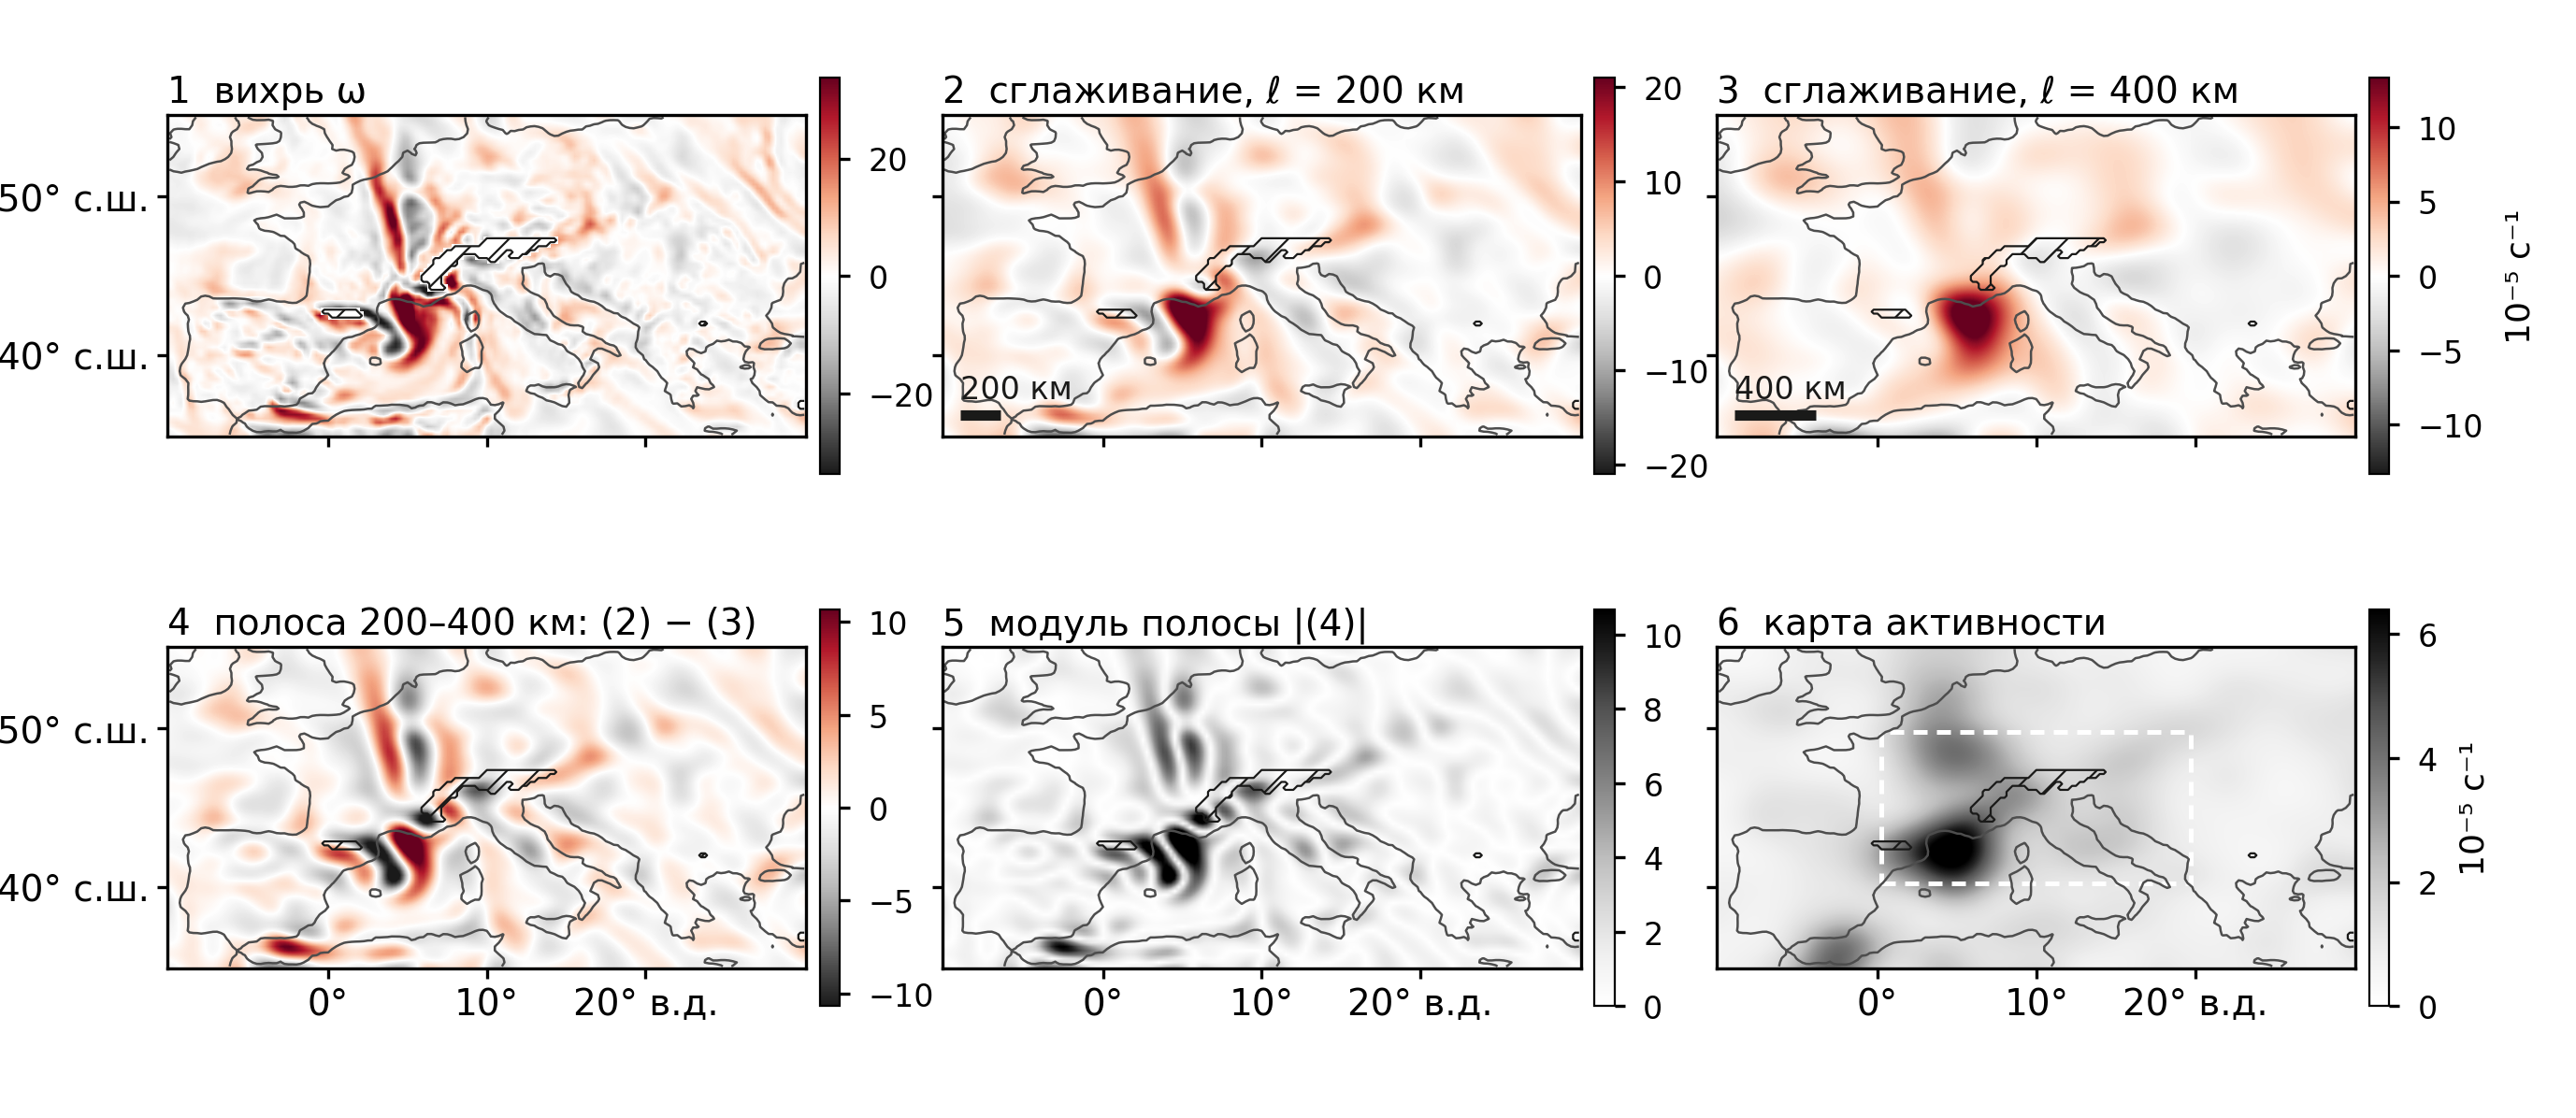
\includegraphics[width=\linewidth]{figures/v8/fig1_method_v8.png}

\noindent Рис. 1. Построение карты активности одной масштабной полосы (шаг 1 методики). Европа, область R11, ERA5, 850 гПа, 3 марта 2024 г., 12 ч ВСВ: 1 -- относительный вихрь $\omega$; 2, 3 -- гауссовы сглаживания с $\ell$ = 200 и 400 км (отрезок -- ширина ядра); 4 -- полоса 200--400 км как разность панелей 2 и 3; 5 -- ее модуль; 6 -- карта активности полосы: модуль, сглаженный с $\ell$ = 400 км. Серые линии -- береговая линия, штриховка -- узлы под рельефом, исключенные из сглаживания и корреляций, пунктир -- внутренняя часть области, по узлам которой вычисляется ранговая корреляция по формуле (3).

\clearpage
\noindent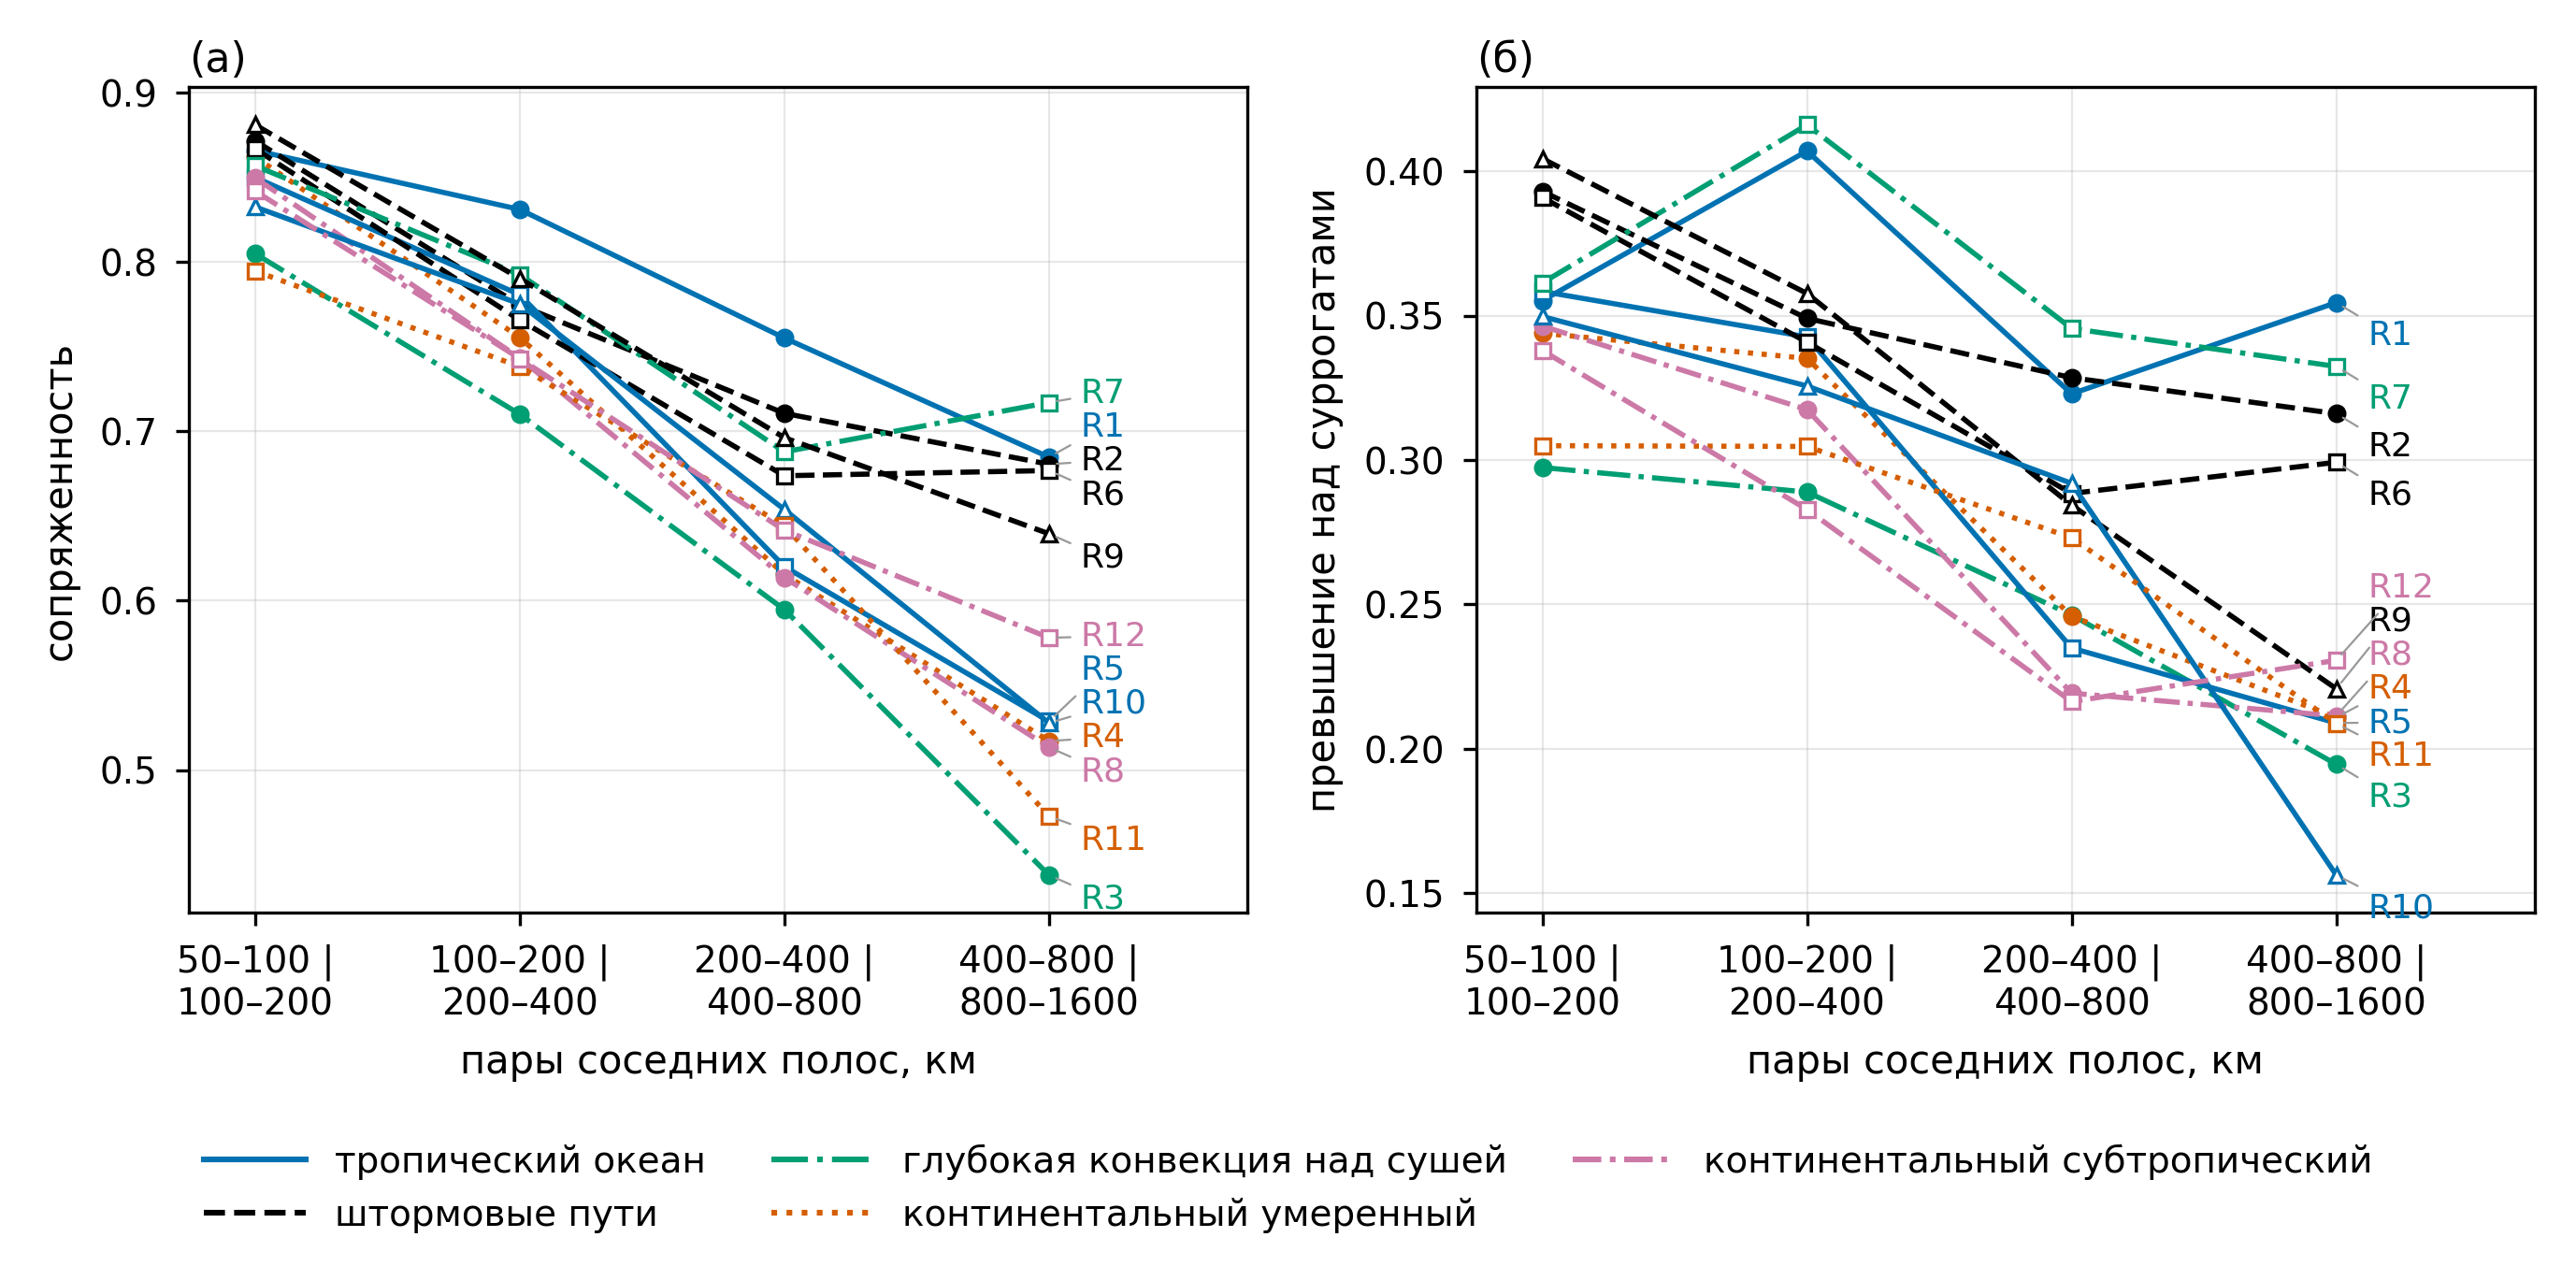
\includegraphics[width=\linewidth]{figures/v8/fig2_profiles_v8.png}

\noindent Рис. 2. Профили сопряженности двенадцати основных областей (коды -- табл. 1) по ступеням 2--5. а -- исходный профиль $P$ на градусных областях, медиана по восьми сезонным окнам 2017--2024 гг.; б -- профиль с суррогатной поправкой $\tilde P$ на равновеликих областях, медиана по четырем окнам 2023--2024 гг. Ступени -- пары соседних полос масштаба, км.

\clearpage
\noindent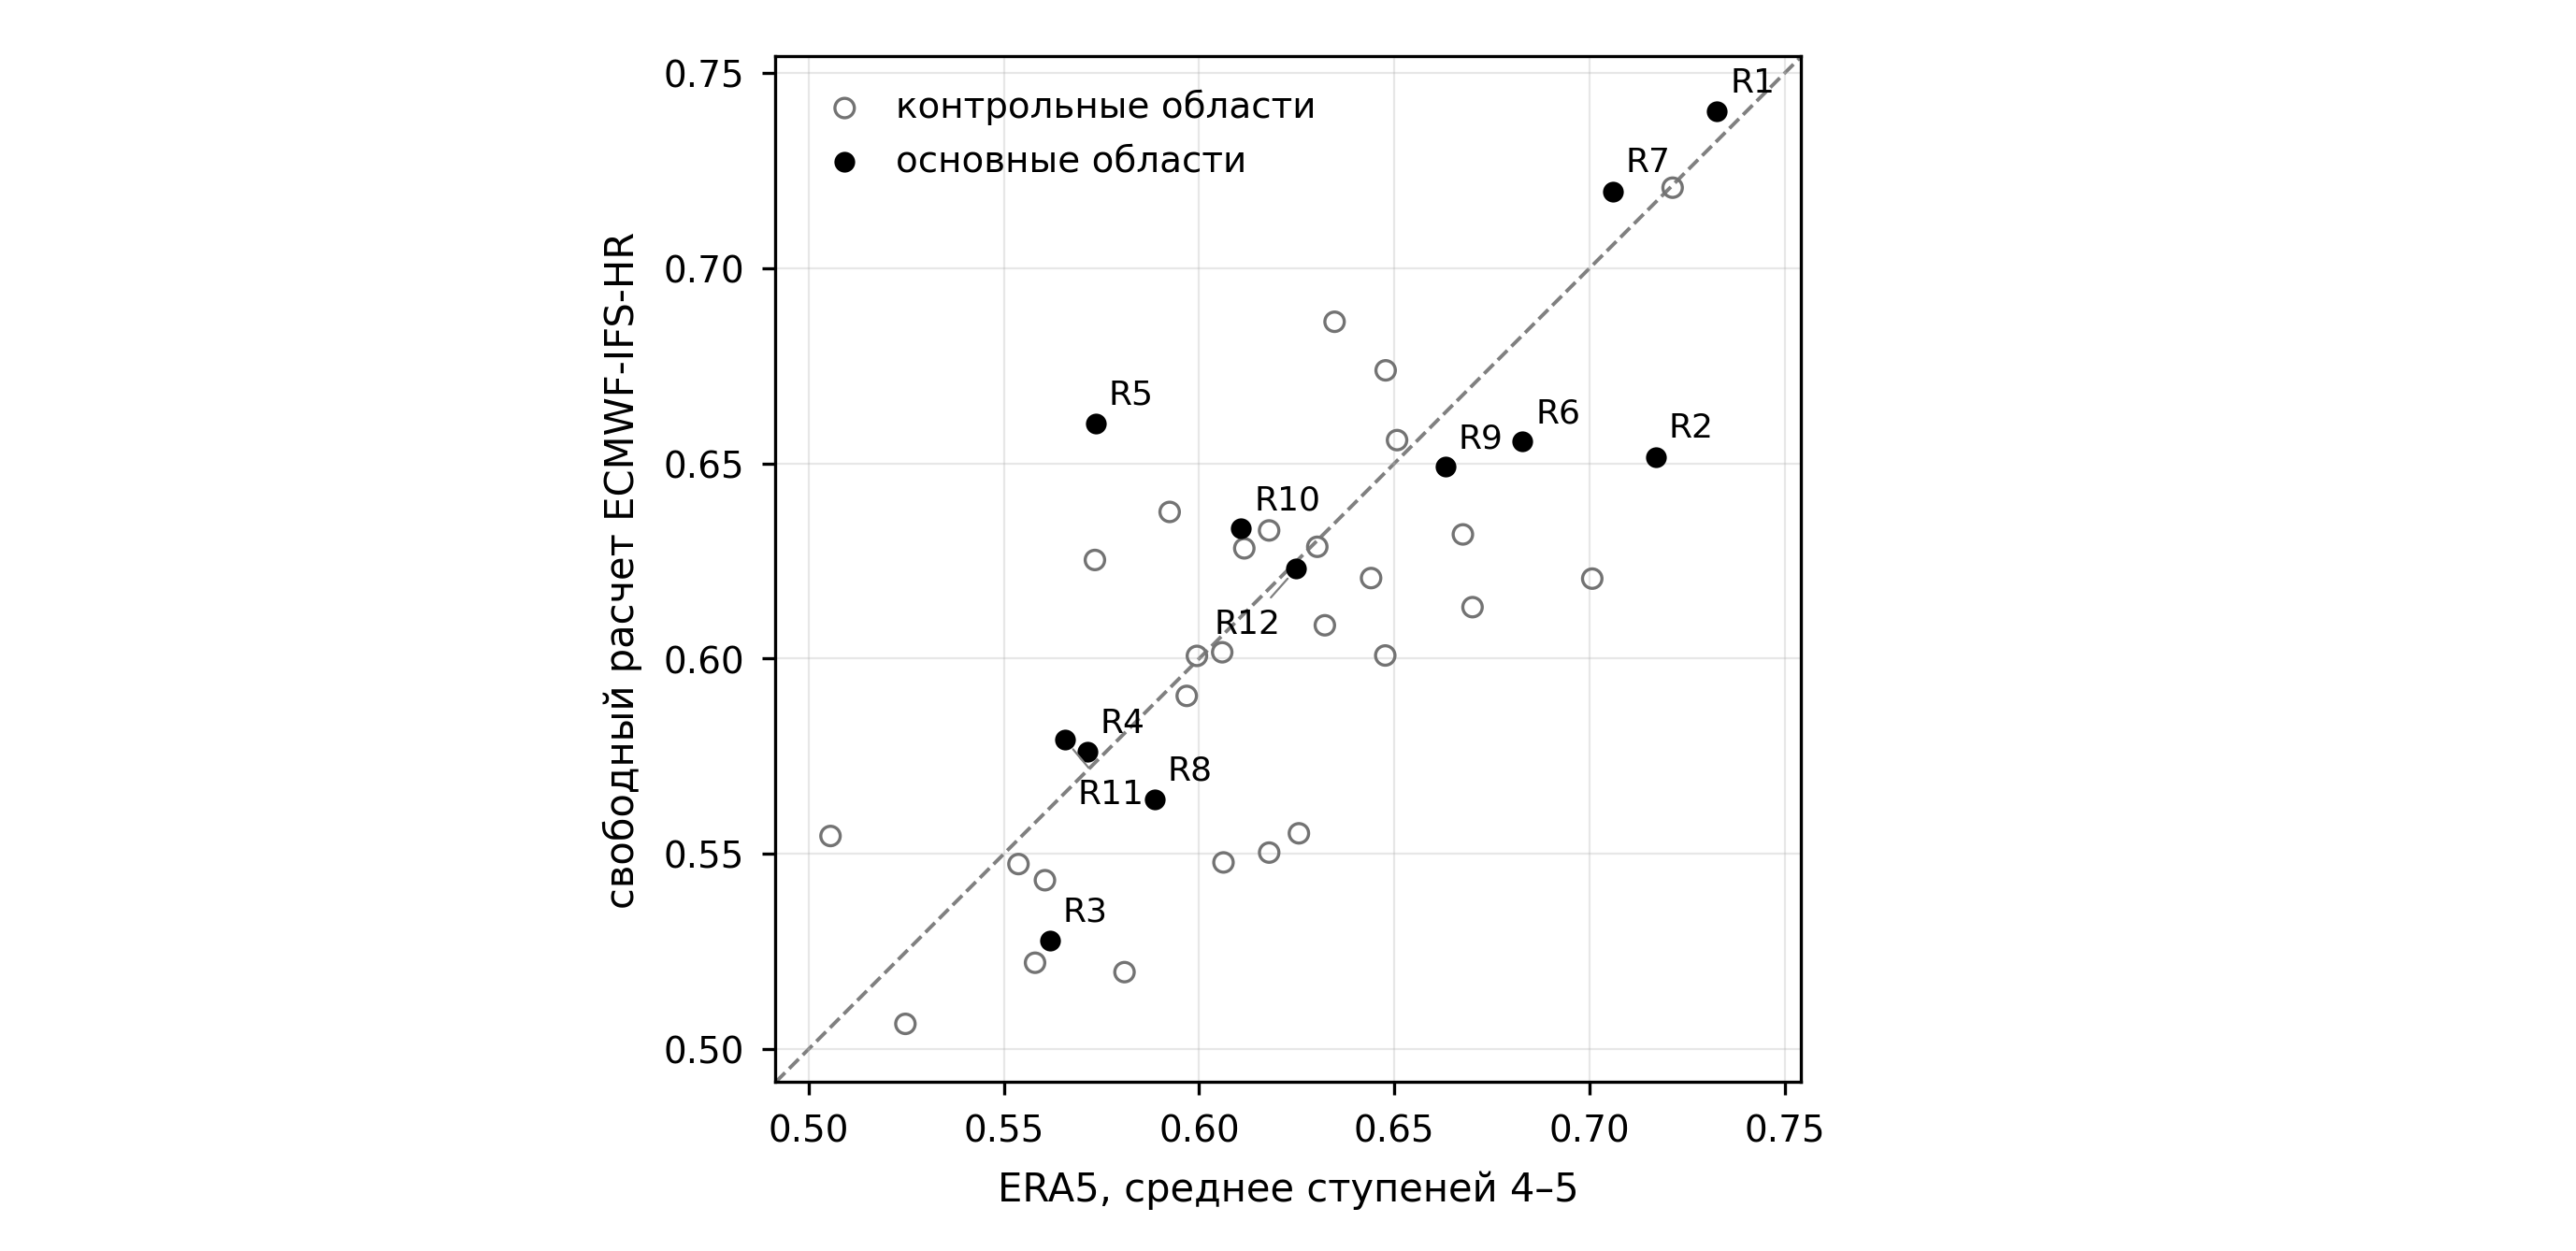
\includegraphics[width=\linewidth]{figures/v8/fig3_free_run_v8.png}

\noindent Рис. 3. Сопоставление региональной географии сопряженности (среднее исходного профиля по ступеням 4--5) по ERA5 (ось абсцисс; окна 2021--2024 гг.) и по свободному расчету ECMWF-IFS-HR без усвоения наблюдений (ось ординат; окна 2014 г.) для 39 областей: заполненные значки -- двенадцать основных областей, полые -- 27 решеточных ячеек; пунктир -- линия равенства.

\clearpage
\noindent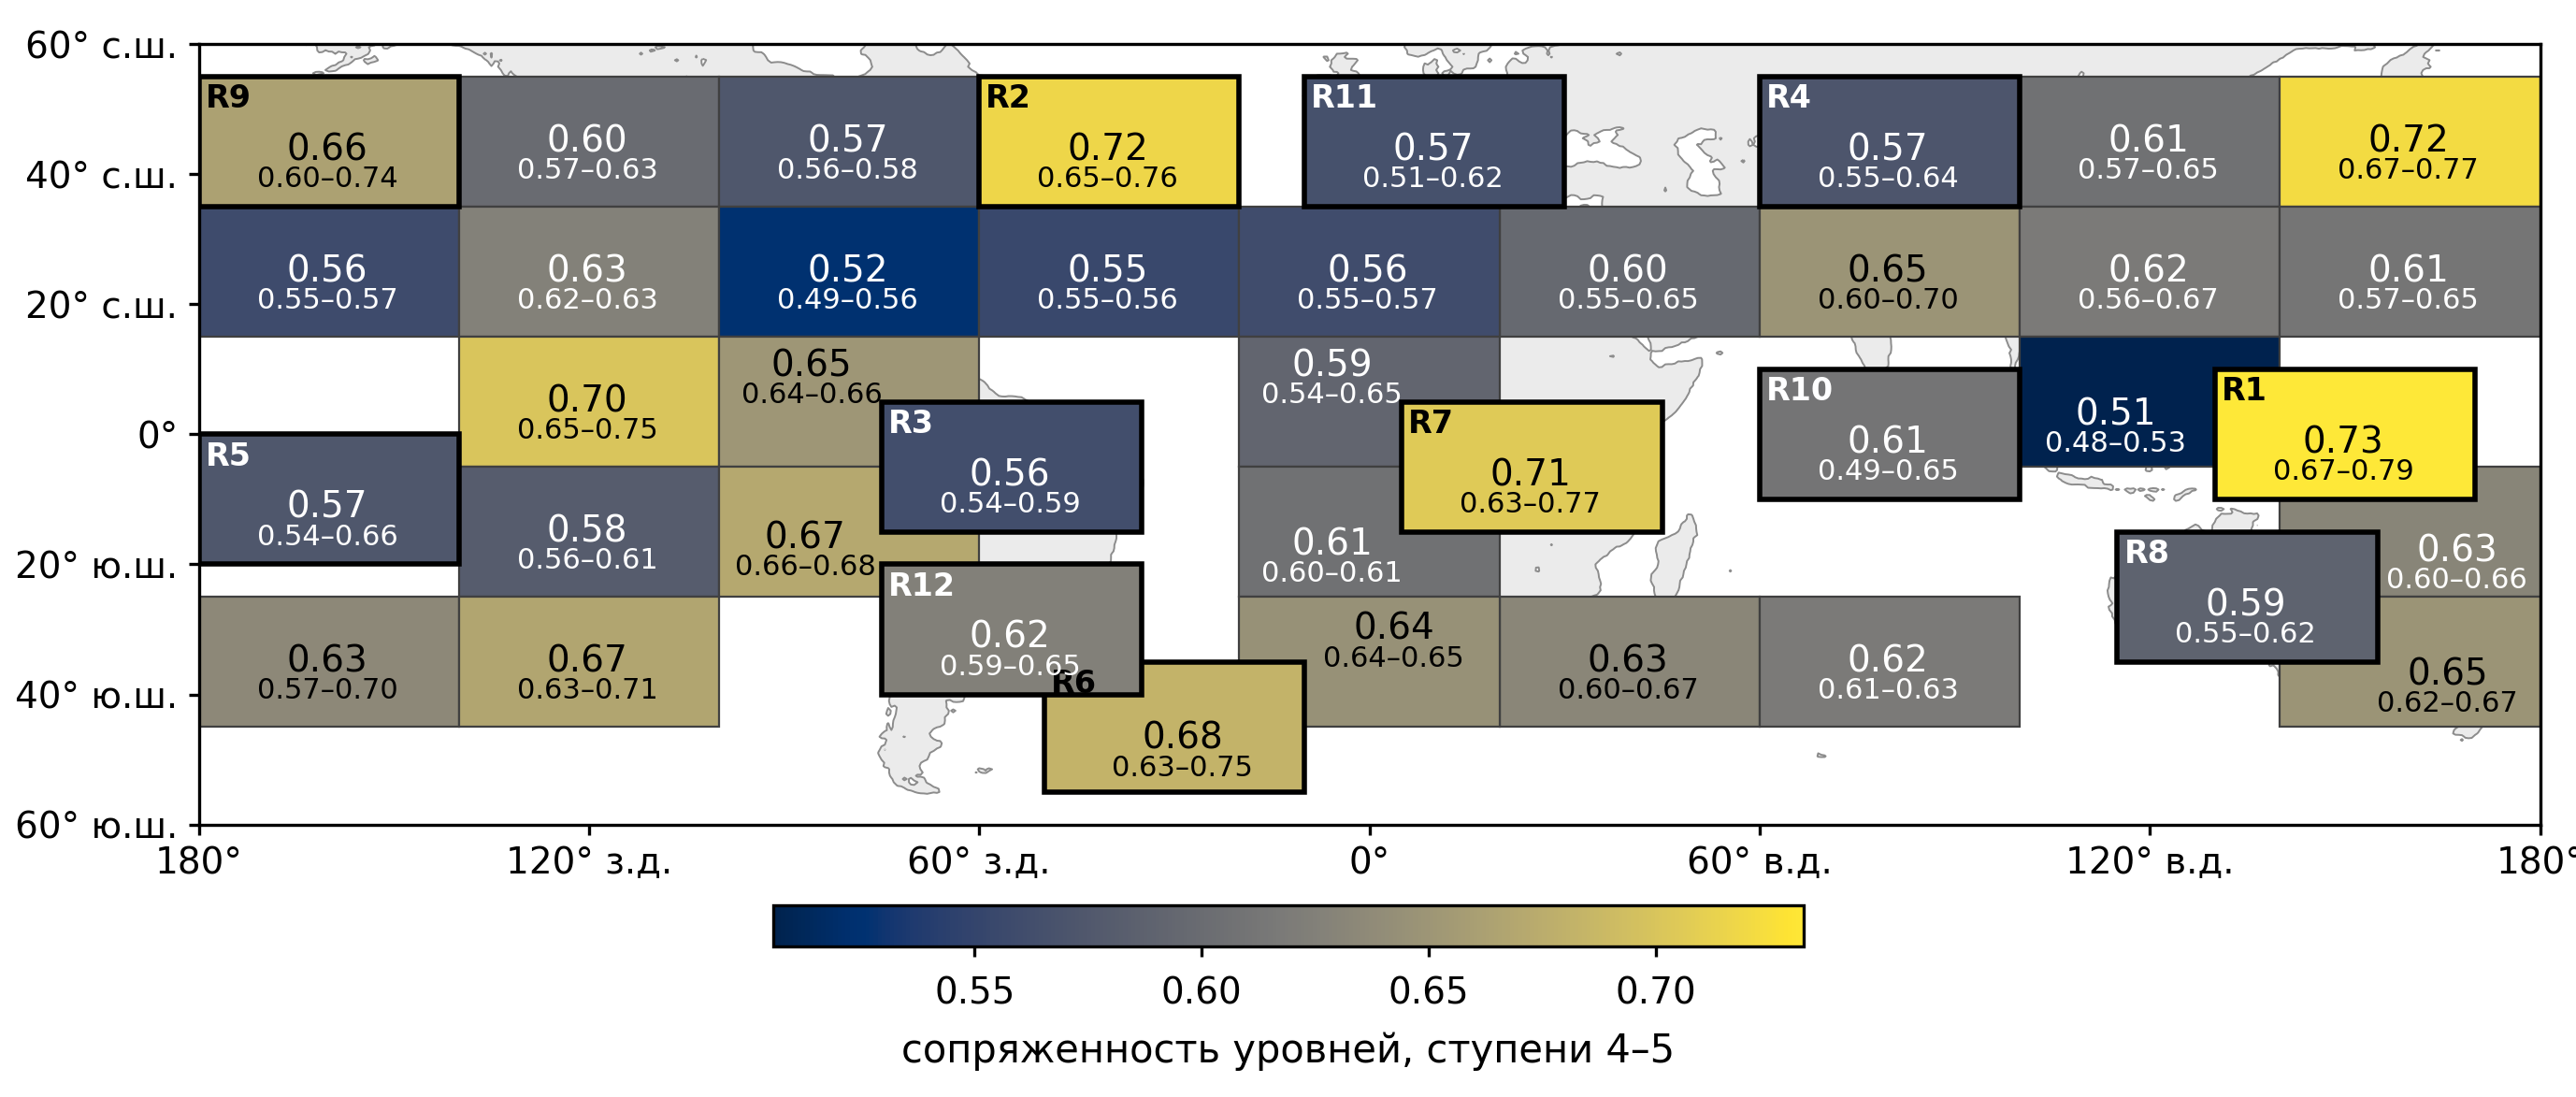
\includegraphics[width=\linewidth]{figures/v8/fig4_map_v8.png}

\noindent Рис. 4. География сопряженности уровней: среднее исходного профиля по ступеням 4--5 (пары полос 200--400 | 400--800 и 400--800 | 800--1600 км) для 39 областей, ERA5, 850 гПа. Каждая область показана отдельным полигоном без интерполяции: число -- медиана по сезонным окнам, под ним -- размах по окнам; двенадцать основных областей (жирная рамка, коды) -- окна 2021--2024 гг. (R1--R4 -- 2023--2024 гг.), 27 решеточных ячеек -- окна 2024 г.

\clearpage
\noindent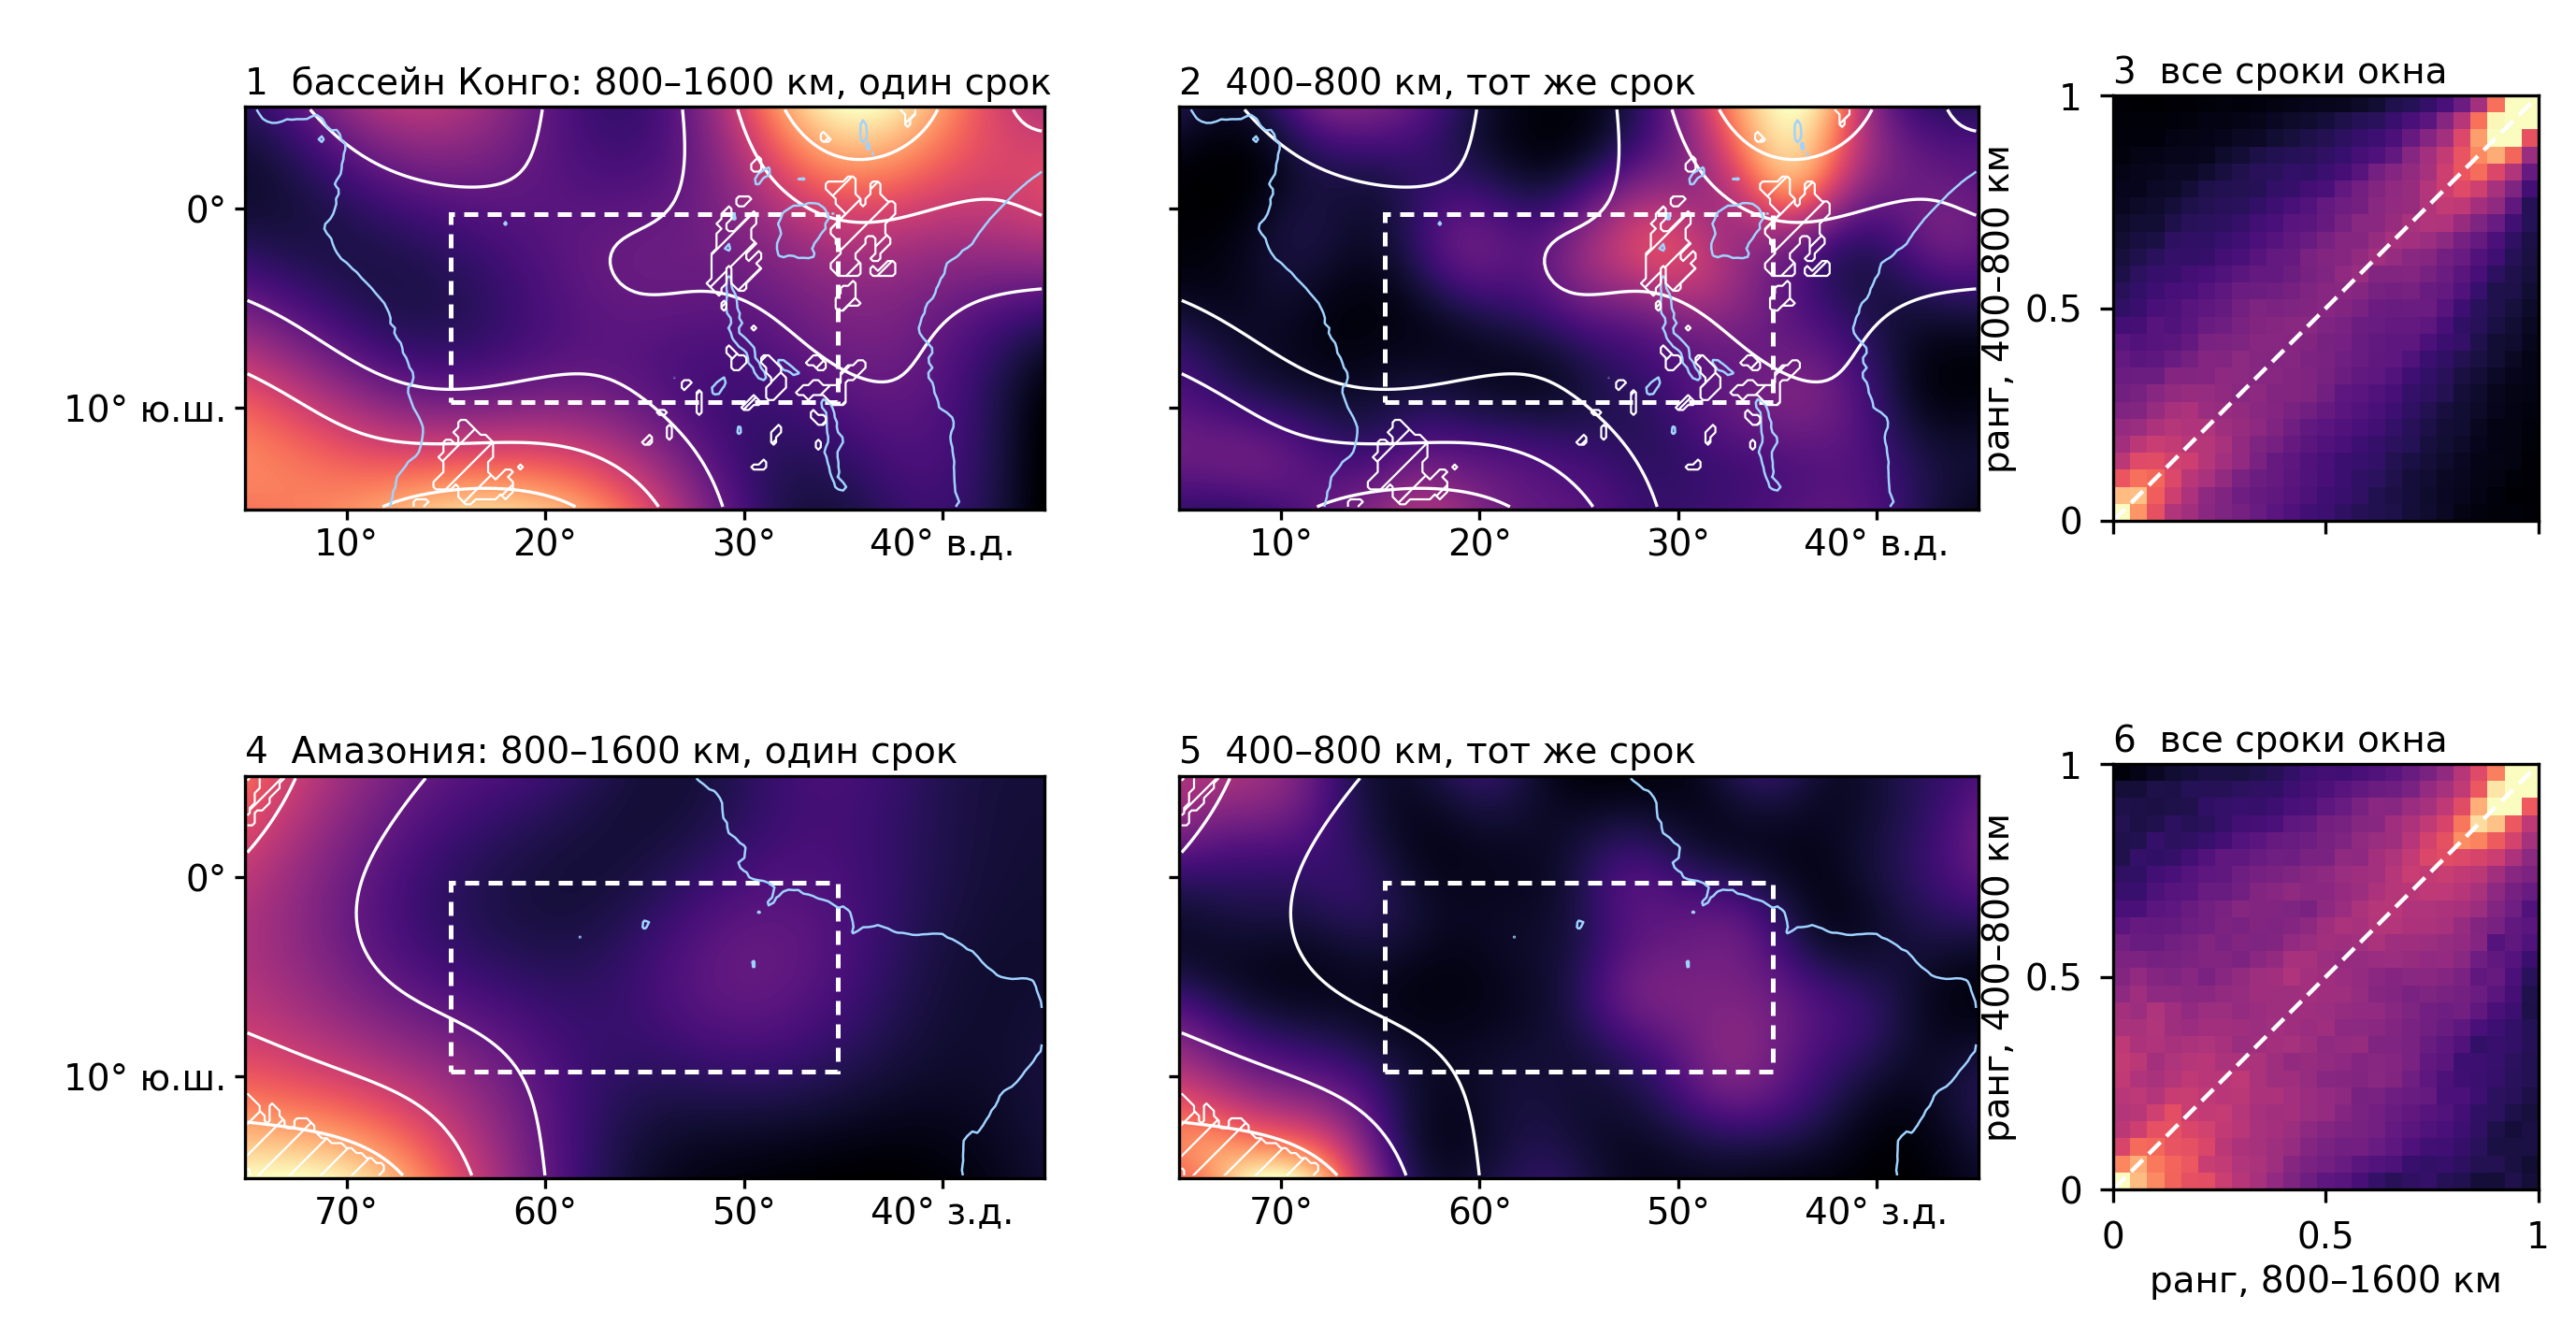
\includegraphics[width=\linewidth]{figures/v8/fig5_congo_amazon_v8.png}

\noindent Рис. 5. Бассейны Конго (1--3) и Амазонки (4--6), январь--март 2023 г. 1, 4 -- карта активности полосы 800--1600 км на один срок (28 февраля 2023 г., 06 ч ВСВ и 15 марта 2023 г., 18 ч ВСВ); 2, 5 -- карта активности полосы 400--800 км на тот же срок; изолинии на обеих картах ряда -- активность полосы 800--1600 км; пунктир -- внутренняя часть области, штриховка -- узлы под рельефом. 3, 6 -- совместное распределение рангов активности двух полос по узлам внутренней части за все сроки окна (темнее -- чаще); пунктир -- диагональ полного соответствия. В бассейне Конго мезомасштабная активность размещается там же, где активен крупный уровень, в Амазонии та же пара уровней распределена почти безразлично.

\clearpage
\begin{center}
{\large\bfseries Coupling of hierarchical levels of the atmospheric circulation as a regional invariant}

\medskip
{\bfseries N. S. Sotiriadi\textsuperscript{*}}

Independent researcher, Moscow, Russia

\textsuperscript{*}E-mail: n.sotiriadi@gmail.com
\end{center}

\begin{singlespace}
\noindent\textbf{Abstract.} Spectral and fractal analysis of geographical fields answers the question of the scales at which the levels of organisation of a geosystem are located. The next question concerns the relation between levels: is mesoscale variability placed where the adjacent large level is active, or independently of it? Using the relative-vorticity field at 850 hPa (ERA5 reanalysis, 2017--2024; 12 main and 27 control regions) we construct a measure of this relation, the coupling profile of adjacent octave scale bands: the spatial rank correlation of the activity maps of two adjacent bands, supplemented by its excess over phase surrogates of the field. We test the hypothesis that the profile is a regional invariant: it distinguishes circulation regimes and is reproduced across seasonal windows of different years and ENSO phases. The regional grouping of profiles is confirmed on held-out windows and under permutations within strata of season, year and period; the region accounts for 0.6--0.7 of the profile variance. The grouping survives restriction to the resolved steps, an equal-area partition, a second reanalysis and a free-running model integration without assimilation of atmospheric observations. Higher values belong to the tropical warm pool of the Pacific, the Congo basin and the extratropical storm tracks, lower values to continental regions and the Amazon; the Congo and Amazon basins, similar in standard regime characteristics, differ in the coupling of their large bands. The quantity adds to regionalisation a characteristic of inter-level relations; its limits of applicability are stated explicitly.

\smallskip
\noindent\textbf{Keywords:} hierarchical organisation of geosystems, invariants of a dynamic geosystem, scale, mesoscale variability, storm tracks, deep convection, reanalysis, regionalisation, falsification design.

\smallskip
\noindent\textbf{Funding.} The study received no external funding. The author declares no conflict of interest.
\end{singlespace}

\end{document}
